% Sanity Checks for Reinforcement Learning Explanations
%
% Self-contained two-column format. To target a specific venue, replace the
% documentclass and geometry block with that venue's style file; the body needs
% no changes.
%
% Length: about ten and a half pages of body, with the bibliography running to
% twelve. That suits arXiv or a journal. For a conference limit of eight pages
% excluding references, cut in this order, which is by how much each section
% would cost in review if it were missing:
%
%   1. the horizon experiment (5.7). it tests a hypothesis that was rejected
%      and superseded by the initialisation identity, so it now documents a
%      dead end rather than supporting a claim.
%   2. the certified-ranking subsection (5.4). the point survives as one
%      sentence in the limitations.
%   3. the integrated-gradients comparison in 5.7, keeping its conclusion.
%
% Do not cut the null-construction audit (5.10) or the rejected-hypotheses
% ledger (5.9) for length. They are the parts a sceptical reader checks first.
%
% Build:  tectonic main.tex

\documentclass[10pt,twocolumn]{article}

\usepackage[letterpaper,margin=0.75in,columnsep=0.28in]{geometry}
\usepackage[T1]{fontenc}
\usepackage[utf8]{inputenc}
\usepackage{amsmath,amssymb}
\usepackage{graphicx}
\usepackage{booktabs}
\usepackage{microtype}
\usepackage{caption}
\usepackage[hidelinks]{hyperref}
\usepackage[numbers,sort&compress]{natbib}
\usepackage{titlesec}
\usepackage{enumitem}
\usepackage{xcolor}
\makeatletter
\makeatother

\captionsetup{font=small,labelfont=bf,skip=4pt}
\titlespacing*{\section}{0pt}{8pt}{4pt}
\titlespacing*{\subsection}{0pt}{6pt}{3pt}
\setlength{\parskip}{0pt}
\setlength{\abovedisplayskip}{5pt}
\setlength{\belowdisplayskip}{5pt}
% the results tables are 4 numeric columns in a 3.35in column. at the 6pt
% default several of them overrun the text block.
\setlength{\tabcolsep}{3.5pt}

\newcommand{\vfn}{v}

\title{\vspace{-1.5em}\bfseries Sanity Checks for Reinforcement Learning Explanations}

% Replace with the venue's anonymous block if submitting double-blind.
\author{Aaryan Singh\\[2pt]
  \normalsize Independent Researcher\\[1pt]
  \normalsize\texttt{singha9@rose-hulman.edu}}
\date{}

\begin{document}

% abstract spans the full page width, as in standard ML conference formats
\twocolumn[
  \begin{@twocolumnfalse}
  \maketitle
  \begin{quote}
  \small
  \textbf{Abstract.}
Interpretability is proposed as a basis for oversight: if we can see which
inputs drive a policy, we can decide whether to trust it. That argument needs
attributions to carry information about the agent, and we show they need not.
On a prediction market that is empirically efficient, a PPO agent whose return
is statistically indistinguishable from abstention produces attributions with a
cross-seed rank correlation of $0.849$, unanimous agreement on the most
important feature, and a top-5 ranking whose adjacent gaps exceed their own
standard errors. Every conventional check passes and the explanation is empty.
We introduce a null-model test that detects this, built on the additivity
identity attribution schemes already satisfy: compare an agent's attribution
span against the spans of agents trained where the observation channel carries
no information. It rejects a planted signal at $z=12.27$, fails to reject the
market agent at $z=+0.23$, and fires at $z=+3.40$ on a genuinely learnable task
built from the same real episodes, so it separates tasks by whether their
observations carry usable information rather than by whether the corpus is
synthetic. Two results then concern practice. Explanations are cheap to forge:
an auxiliary training penalty drives a feature's attribution from $39.9\%$ to
$3.2\%$ of total mass at no measurable cost in return, with no deception and no
attack on the explainer, so an oversight regime reading attributions as
evidence of what a model relies on is reading a quantity the developer can set
wherever the feature does not matter. And the established sanity check for this
purpose, randomising network parameters, does not transfer to reinforcement
learning: across sixteen checkpoints on four control tasks it never exceeds
$z=2.45$, because its reference distribution equals the spread of
random-initialisation return to three significant figures and therefore
measures the variance of initialisation, not the explanation.
  \end{quote}
  \vspace{1.2em}
  \end{@twocolumnfalse}
]

\section{Introduction}

A common argument for interpretability is oversight: if we can see which inputs
drive a policy, we can decide whether to trust it. This requires that an
attribution mean something. It is not obvious that attributions do, and it is
less obvious how one would tell.

The difficulty is that attribution methods return an answer regardless. Given any
policy and any state, Shapley values~\citep{shapley1953value,lundberg2017unified},
integrated gradients~\citep{sundararajan2017axiomatic}, and permutation
importance all produce a vector of numbers, ranked, signed, and plottable.
Nothing in the output distinguishes an attribution reflecting structure the agent
exploits from one reflecting nothing at all.

In supervised learning this is handled by randomisation tests.
\citet{adebayo2018sanity} compare explanations of a trained model against
explanations of a model with randomised parameters, and against a model trained
on permuted labels. If the explanation does not change, it does not depend on
what the model learned. These tests are standard, and applying them invalidated
several saliency methods.

Reinforcement learning has adopted only half of this.
\citet{huber2022benchmarking} apply the parameter-randomisation test to saliency
maps for Atari agents, and observe that the data-randomisation test has no
obvious RL analogue: there is no labelled dataset to permute, and it is unclear
how a sequential decision maker should respond to artificially corrupted
features.

This paper supplies that analogue, and shows that the half already adopted does
not work.

\paragraph{Contributions.}
\begin{enumerate}[leftmargin=1.2em,itemsep=1pt,topsep=2pt]
\item \textbf{An environment-level null for RL.} Rather than corrupting the
model or the labels, we corrupt the environment's \emph{observation channel},
leaving dynamics and reward intact. The agent trains normally, on a real
objective, with nothing to condition on, and this requires no access to task
internals (Section~\ref{sec:method}).

\item \textbf{A worked case} of an uninformative explanation passing every
conventional check: stable across seeds, separated beyond its own estimation
error, and legible (Section~\ref{sec:empty}).

\item \textbf{Attribution is not identified by behaviour.} An auxiliary
training penalty drives the market agent's dominant feature from $39.9\%$ to
$3.2\%$ of attribution mass at no measurable cost in return; the same
intervention on a load-bearing feature costs $81\%$ of return. No deception and
no attack on the explainer is involved (Section~\ref{sec:steering}).

\item \textbf{The established null fails in RL, and we show why.} Parameter
randomisation never exceeds $z=2.45$ across sixteen checkpoints, including on a
converged CartPole policy scoring 404 of 500, while the environment null reaches
$z=117$. Its width equals the standard deviation of random-initialisation return
to three significant figures, so it measures the variance of initialisation
(Section~\ref{sec:nulls}).

\item \textbf{Validation with ground truth, synthetic and real.} We construct
environments where the correct attribution is known by construction
(Sections~\ref{sec:synthetic} and~\ref{sec:groundtruth}), and a positive control
on real market episodes where only the objective varies
(Section~\ref{sec:positive}).

\item \textbf{An audit of our own null construction}, which our thesis implies
must matter and does (Section~\ref{sec:nullchoice}).
\end{enumerate}

\paragraph{What we do not claim.}
The argument that RL attribution should target outcomes rather than policy
outputs is due to \citet{beechey2023sverl}, whose SVERL framework unifies
behaviour, outcomes and prediction, and whose FastSVERL~\citep{beechey2025fastsverl}
addresses the scalability, off-policy and temporal problems we only name. Our
test adapts the data-randomisation test of \citet{adebayo2018sanity}.
Deletion-based fidelity evaluation is established practice in
XRL~\citep{cheng2025survey,milani2024xrl}. Our contribution is the RL
construction, the demonstration that the incumbent alternative fails, and the
empirical consequences.

\section{Related work}

\paragraph{Shapley values in RL.}
\citet{beechey2023sverl} give a theoretical account of Shapley-value explanation
for RL, showing that earlier applications explained the wrong object and
proposing characteristic functions built on agent performance. Their framework
identifies three explanatory targets: behaviour, outcomes, and prediction.
FastSVERL~\citep{beechey2025fastsverl} makes the approach tractable and addresses
temporal dependence and off-policy data. We adopt the outcomes framing and
implement it independently; we do not extend the theory.

\paragraph{Sanity checks.}
\citet{adebayo2018sanity} introduced parameter- and data-randomisation tests;
\citet{binder2023shortcomings} examine their limitations.
\citet{huber2022benchmarking} apply the parameter test to perturbation-based
saliency for Atari agents and note the data test lacks an RL analogue. We propose
one, and show the parameter test is the weaker of the two in this setting.

\paragraph{Manipulating explanations.}
\citet{slack2020fooling} construct adversarial classifiers that detect the
off-manifold points LIME and SHAP query and behave differently on them, yielding
innocuous explanations for biased models. That is an attack on the explainer's
sampling. Our steering result differs in kind: we train a normal agent with an
invariance penalty, the resulting explanation is \emph{correct} about the
resulting model, and the point is that behaviour does not pin the explanation
down. It is a non-identifiability result rather than an attack.

\paragraph{Uncertainty in Shapley estimation.}
\citet{goldwasser2024significance} certify top-$k$ Shapley rankings against Monte
Carlo error. These guarantees concern the estimator. Section~\ref{sec:certified}
shows they are orthogonal to whether the explained model learned anything.

\paragraph{Evaluation in XRL.}
Surveys note that the absence of ground-truth explanations is a central obstacle,
and that perturbation-based fidelity is the common
recourse~\citep{cheng2025survey,milani2024xrl}. We use deletion curves in that
established sense and do not claim them as a contribution.

\section{Method}
\label{sec:method}

\subsection{The statistic}

Let $\vfn(S)$ be the expected episode return of an agent observing only the
features in $S \subseteq N$, with features outside $S$ replaced at every timestep
by draws from a reference distribution. Define the \emph{attribution span}
\begin{equation}
\Delta \;=\; \vfn(N) - \vfn(\emptyset).
\end{equation}

Shapley values~\citep{shapley1953value} and integrated
gradients~\citep{sundararajan2017axiomatic} satisfy additivity identities
(efficiency and completeness respectively) under which per-feature attributions
sum to $\Delta$. The span can therefore be read off either.

It is worth stating precisely what $\Delta$ is. It is \emph{not} a Shapley
quantity: it is the difference between two masked rollouts, and depends only on
the masking scheme. Efficiency tells us the Shapley values happen to sum to it.
This has a practical consequence we exploit: $\Delta$ costs two evaluations
rather than $2^{|N|}$.

\subsection{The null}

The test compares an observed $\Delta$ against the distribution of $\Delta$ for
agents that had nothing to learn. We construct these by corrupting the
observation channel (Figure~\ref{fig:method}).

\begin{figure*}[t]
\centering
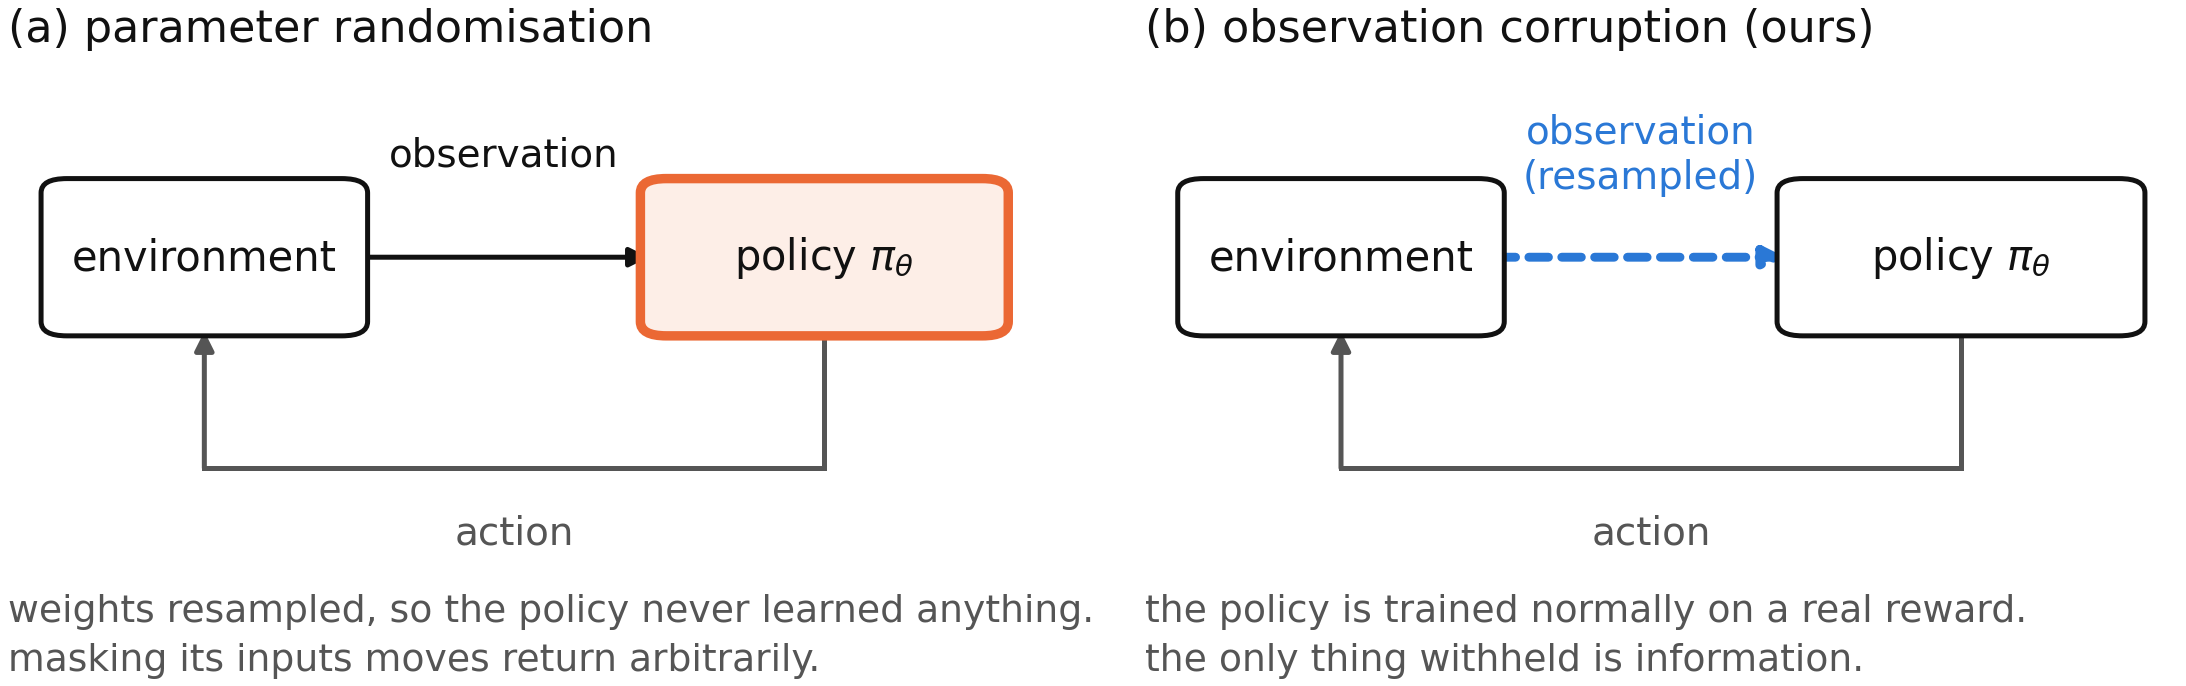
\includegraphics[width=\textwidth]{figures/fig_method.png}
\caption{Two ways to build a reference distribution of explanations for an agent
that learned nothing. The established check (a) randomises the policy's
parameters, leaving a network that was never trained. Ours (b) leaves the policy
and its training untouched and corrupts the environment's observation channel,
so the agent optimises a real reward with nothing to condition on. Only (b)
yields a normally trained policy, which is the failure mode that occurs in
deployment; Section~\ref{sec:nulls} shows the difference is worth $42\times$ in
the width of the resulting reference distribution.}
\label{fig:method}
\end{figure*}

\medskip
\noindent\textbf{Blind-observation null.} \emph{Replace every observation with an
independent draw from a fixed reference distribution matched to the
environment's observation moments. Leave dynamics and reward untouched. Train
normally.}
\medskip

Such an agent faces the real task and receives real return; it simply cannot
condition on anything. This is the RL counterpart of training on permuted labels,
and unlike parameter randomisation it yields a \emph{normally trained} policy:
the failure mode that occurs in deployment rather than an artificial one.

Matching the reference moments matters. A network fed out-of-range inputs fails
for reasons of scale rather than information, which would be a different
experiment.

\subsection{The test}

Given $\Delta_{\mathrm{obs}}$ and null draws $\Delta_1,\dots,\Delta_n$ with mean
$\bar\Delta$ and standard deviation $s$, we report
% set on two lines: side by side these overrun the column by 18pt.
\begin{align}
p_{\mathrm{rank}} &= \frac{\#\{i : |\Delta_i - \bar\Delta| \ge |\Delta_{\mathrm{obs}} - \bar\Delta|\} + 1}{n+1}, \\[2pt]
z &= \frac{\Delta_{\mathrm{obs}} - \bar\Delta}{s},
\end{align}
and require both to reject.

Two statistics are reported because neither suffices. The rank statistic assumes
no distributional shape but bottoms out at $1/(n+1)$: with $n=8$ it cannot reject
at $\alpha=0.05$ however extreme the observation, and in an early run it reported
$p=0.111$ for a signal lying $10.5$ standard deviations outside the null. The
normal statistic has resolution but assumes a shape the null need not have.
Requiring both keeps the test conservative in the direction that matters.

\paragraph{Degenerate nulls.} If every null draw is identical, $s=0$ and $z$ is
undefined. We return $z=\pm\infty$ and surface the degeneracy rather than
guarding it away, because silently returning $z=0$ would convert an
overwhelming result into a null one.

It is tempting to read a degenerate null as maximally informative, since any
deviation from a point mass is infinitely surprising. An earlier version of this
paper said exactly that, and Section~\ref{sec:matched} shows it is wrong: a
point-mass null has no specificity, and we produce a false positive with one on
a corpus that provably contains no signal. Degeneracy is a defect of the
construction and a reason to distrust the reference, not a strong result. It
occurs whenever a task lets the null agents converge on a single behaviour,
which is a property of the null construction rather than of the agent under
test.

\section{Experimental setup}

\subsection{Environments with known answers}
\label{sec:synthetic}

Explanation evaluation lacks ground truth~\citep{cheng2025survey}. We construct
three synthetic corpora in which the correct answer is fixed by construction.
Episodes are fixed-length with no early termination, so the horizon is controlled
exactly.

\begin{itemize}[leftmargin=1.1em,itemsep=1pt,topsep=2pt]
\item \textbf{Planted signal.} One of 18 features is informative about the binary
outcome; the rest are noise or constants.
\item \textbf{Null.} Identical shapes and frictions, no informative feature. The
optimal policy is to abstain.
\item \textbf{Decoy.} One feature correlates $0.989$ with the outcome in the first
$60\%$ of episodes and $0.006$ in the remainder.
\end{itemize}

The claim about the planted corpus needs care. The planted feature is the only
one informative about the \emph{outcome}. Others can still affect the
\emph{return} without predicting anything, because return depends on behaviour:
an agent that cannot tell where it is in an episode acts incoherently and pays
transaction costs. The test is that the planted feature ranks first with the
majority of attribution mass, not that everything else is zero.

\subsection{A market with terminal ground truth}
\label{sec:market}

Our main empirical setting is a binary contract settling to \$1.00 if BTC is
higher after 15 minutes and \$0.00 otherwise, on a regulated prediction market.
We use 6{,}425 settled contracts over 68 days (89{,}950 transitions, outcome rate
$0.4999$), with a walk-forward split by time and purge gaps; the test split is
evaluated once.

This instrument was chosen for one property: every episode resolves to a known
value, so a critic's $V(s)$ can be checked against realised settlement frequency.
Agents are trained with PPO~\citep{schulman2017ppo}. State is 18 causal
features. Actions are target inventory in
$\{-1,0,+1\}\times q_{\max}$. Reward is the change in mark-to-market equity net
of costs, which telescopes exactly to net episode P\&L.

Transaction costs use the exchange's published taker schedule,
$\lceil 0.07\,C\,P(1-P)\rceil$, maximised at $P=0.5$ where this contract trades by
construction. With the measured one-cent modal spread this is a $9\%$ round-trip
hurdle on a 50-cent notional, and it determines most of what follows.

\subsection{Control tasks}

CartPole-v1 (4 features), Acrobot-v1 (6), MountainCar-v0 (2) and Pendulum-v1
(3) provide settings with no relationship to trading and well-understood optimal
policies. All four have observation spaces small enough to enumerate every one
of the $2^{|N|}$ coalitions, so per-feature Shapley values there are exact.
Pendulum's action space is continuous; we discretise it into nine evenly spaced
values so the same categorical PPO trains on every task, at the cost of fine
control near the optimum.

\subsection{Reproducibility}

All results derive from public endpoints with no API keys. Hyperparameters were
fixed a priori from synthetic sweeps where the correct answer is known
analytically, not tuned on validation performance. The full pipeline is one
command; 235 tests cover the environment, the attribution implementations, and
six no-lookahead properties verified by mutation testing. Every numerical claim
in this paper is asserted against its source artifact by a script that runs as
the pipeline's final stage.

\paragraph{Code and compute.} Code, data-ingest scripts and the exact commands
that produce every figure and table are at
\url{https://github.com/Aaryansi/nano-l1}. All experiments run on CPU: an
8-core Apple M1 with 8\,GB of memory, no GPU at any stage. The complete pipeline
takes roughly two hours from a cold cache, of which about 27 minutes is
rate-limited market ingest, and roughly one hour warm. Policies are two-layer
MLPs of 64 hidden units; the 18-feature market agent has 5{,}636 parameters. The
headline experiments are therefore reproducible on a laptop, which is a
deliberate property of the setting rather than an accident: the claims concern
whether an explanation carries information, and that question does not require
scale to pose.

\paragraph{Hyperparameters.} PPO with clipped surrogate, GAE, and
$\gamma=1.0$; $\gamma$ is unity because episodes are finite-horizon and reward
telescopes exactly to terminal P\&L, so discounting would bias the objective
away from the quantity of interest. Market agents train for 100 updates over 5
seeds; explanation-time agents for 60 updates; null draws use $n=24$ for the
main test and 12--16 for the environment and robustness experiments. Full
values, including network widths, learning rate, clip range and entropy
coefficient, are in the configuration files in the repository rather than
restated here.

The exchange serves a moving window, so re-running the ingest returns a different
set of contracts. A cold rebuild five days after the original produced 6{,}425
episodes against 6{,}428, sharing 5{,}960 tickers; \emph{overlapping episodes are
byte-identical on every field}. Ingest is deterministic per contract and what
changes is membership. All conclusions reproduced (Section~\ref{sec:repro}).

\section{Results}

\subsection{An explanation that passes every check and says nothing}
\label{sec:empty}

The market is empirically efficient: its implied probability has a weighted mean
absolute calibration error of $0.0172$ across ten bins, and spot return
correlates $0.476$ with the outcome but only $0.016$ with the residual after the
price is accounted for. No policy beats abstention (Table~\ref{tab:baselines});
losses track turnover.

\begin{table}[t]
\centering\small
\caption{Test split, 1{,}284 held-out episodes. $p$-values are paired bootstrap
against always-flat on the same episodes, necessary because per-episode P\&L has
a standard deviation near 50 against differences near 1.}
\label{tab:baselines}
\begin{tabular}{lrrr}
\toprule
Policy & Mean P\&L & Trades/ep & $p$ vs flat \\
\midrule
always-flat        & $+0.000$  & 0.00 & n/a \\
buy-and-hold       & $-1.608$  & 1.00 & 0.23 \\
\textbf{PPO} (5 seeds) & $\mathbf{-0.595 \pm 0.176}$ & 1.37 & \textbf{0.10} \\
logistic (refit)   & $-5.729$  & 2.52 & $<$0.0001 \\
mean-reversion     & $-11.615$ & 4.94 & $<$0.0001 \\
random             & $-18.532$ & 9.33 & $<$0.0001 \\
\bottomrule
\end{tabular}
\end{table}

PPO's shortfall is its own. On synthetic data containing no signal by
construction the same agent scores $-0.47 \pm 0.47$; here it scores
$-0.595 \pm 0.176$. Nothing is left to attribute to the market.

Yet its explanations look entirely reasonable. Across five seeds whose pairwise
performance differences are statistically indistinguishable in all ten pairs:
behaviour attributions have cross-seed rank correlation $0.849$ (min $0.761$)
with $100\%$ agreement on the top feature and $100\%$ sign agreement; the top-5
ranking is fully certified, all four adjacent gaps exceeding their combined
standard errors; and the ranking is semantically legible, time-to-expiry
dominating, which reads as an agent that learned when not to trade.

The null test disagrees (Table~\ref{tab:null}, Figure~\ref{fig:null}).

\begin{table}[t]
\centering\small
\caption{Null-model test on the market. Null from 24 blind-trained agents,
span $+8.19 \pm 5.11$.}
\label{tab:null}
\begin{tabular}{lrrl}
\toprule
Case & Span & $z$ & Verdict \\
\midrule
planted signal & $+70.89$ & $\mathbf{+12.27}$ & informative \\
null corpus    & $+11.86$ & $+0.72$ & not distinguishable \\
\textbf{real market} & $\mathbf{+9.37}$ & $\mathbf{+0.23}$ & \textbf{not distinguishable} \\
\bottomrule
\end{tabular}
\end{table}

\begin{figure}[t]
\centering
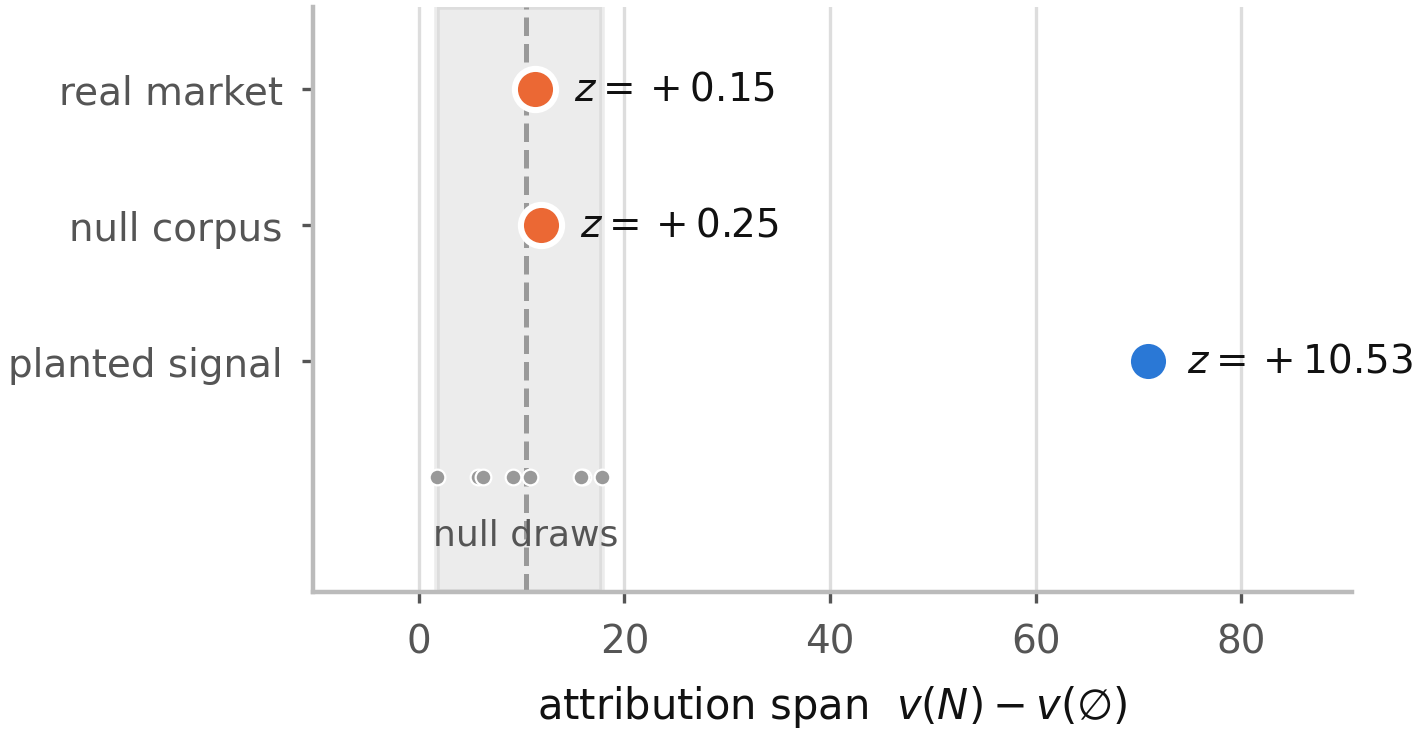
\includegraphics[width=\columnwidth]{figures/fig_null_test.png}
\caption{Attribution spans against the null distribution. The shaded band is the
range over 24 agents trained where the observation channel carries no
information. The market agent sits at its centre.}
\label{fig:null}
\end{figure}

The test has power and specificity. The market agent's explanation sits at the
centre of the distribution of explanations of nothing.

We note one consequence for our own reporting. An earlier draft stated that ``the
whole observation is worth $+5.914$ per episode against being blind'' and
presented it as a finding. Blind agents produce $+8.19 \pm 5.11$. It was noise.

\subsection{Validation against ground truth}
\label{sec:groundtruth}

On the planted corpus, outcome attribution ranks the planted feature first with
$55\%$ of total attribution mass. This check is unavailable on real data and is
what licenses the rest.

On the decoy corpus, an agent trained where the decoy predicts the outcome
(in-sample $+47.24$, held out $-6.83$) is explained on held-out episodes where
the decoy is provably worthless (Figure~\ref{fig:decoy}). Per-decision
attribution of $\pi(a\mid s)$ gives it $6.5\%$ of mass, rank 3 of 18;
outcome-based attribution gives it $1.1\%$, rank 10.

Both statements are true. The policy does key on the decoy, so per-decision
attribution is correct about behaviour and misleading about value. An auditor
asking what an agent relies on that does not work gets the wrong answer from it.

Deletion curves agree: removing features in the order each ranking considers
important, the outcome ranking degrades return faster (AUC $-187.8$ against
$-165.3$; a random ranking gives $+366.6$).

\begin{figure}[t]
\centering
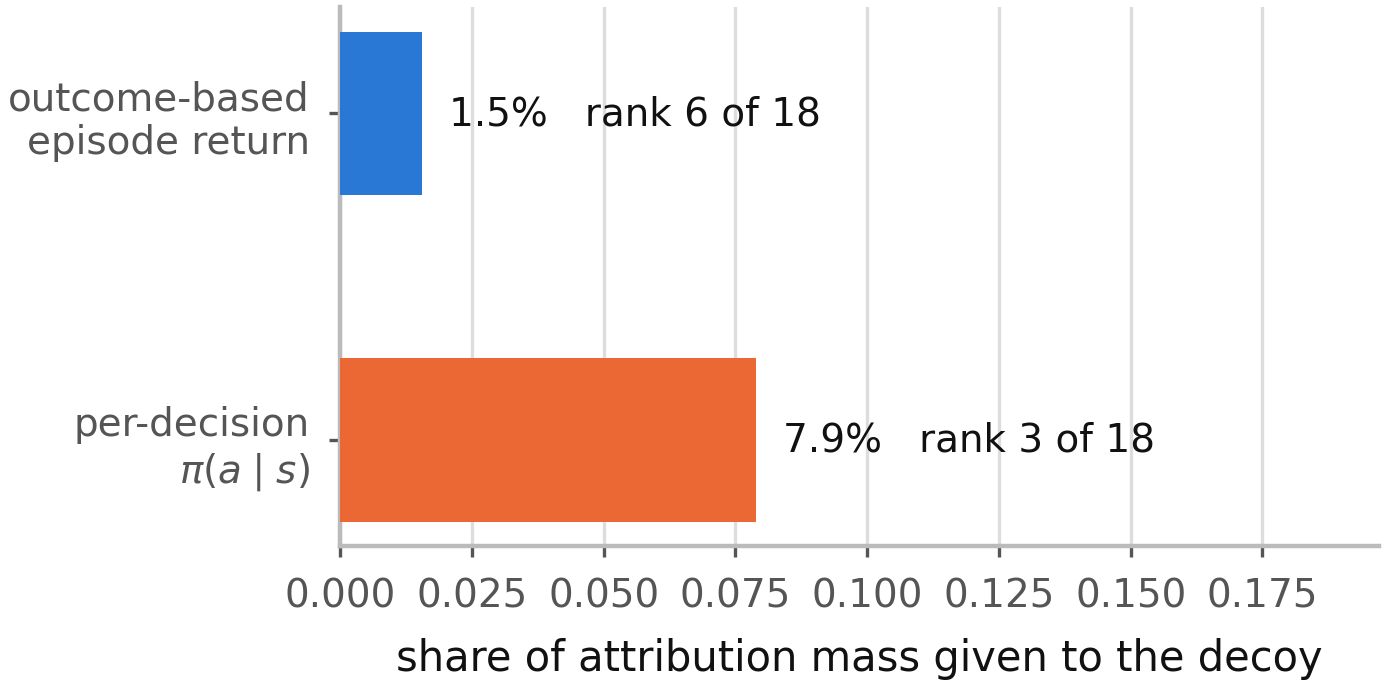
\includegraphics[width=\columnwidth]{figures/fig_decoy.png}
\caption{A feature that drives the policy but earns nothing, on held-out episodes
where it is provably uninformative.}
\label{fig:decoy}
\end{figure}

\subsection{How much edge is required}

Sweeping planted-signal strength calibrates the test (Figure~\ref{fig:power}).
Detection begins near $+3.45$ per episode of \emph{measured} edge. The market
agent earns $-0.595$: an order of magnitude below threshold and of the wrong
sign. These edges are in-sample and therefore optimistic; the threshold is a
lower bound.

\begin{figure}[t]
\centering
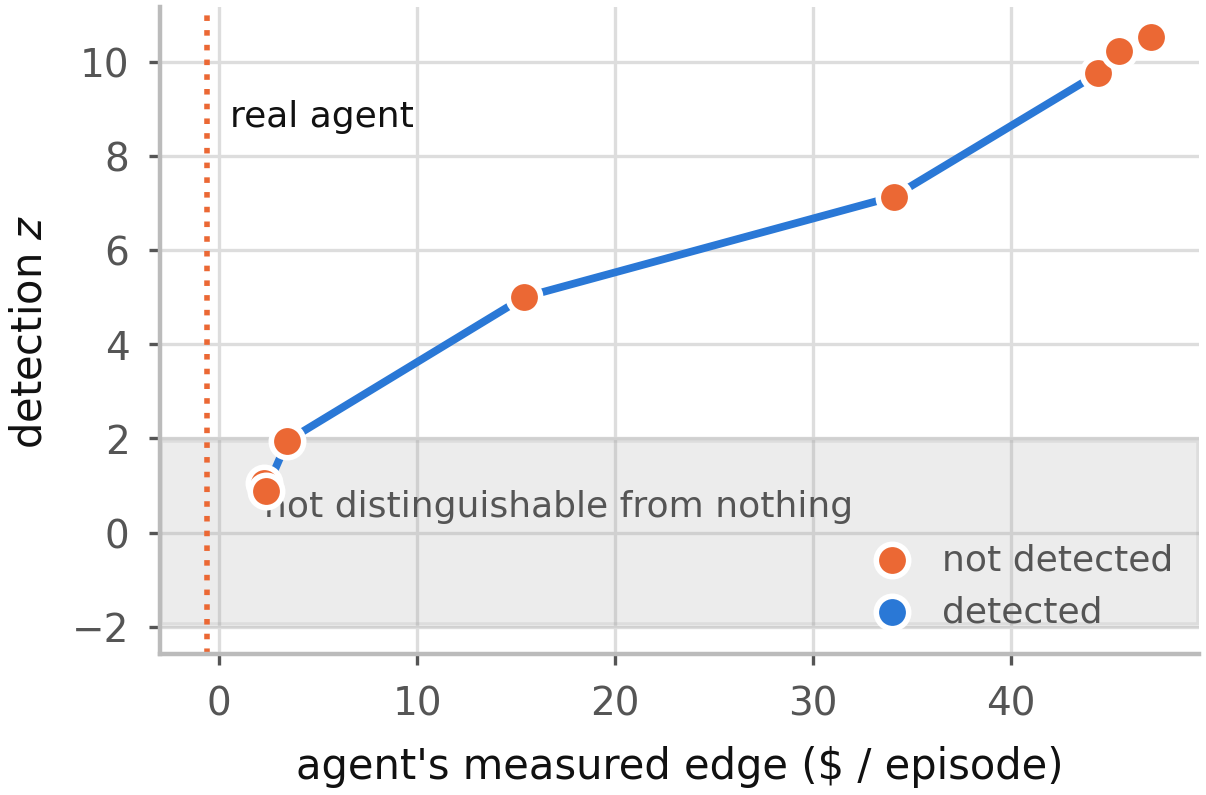
\includegraphics[width=\columnwidth]{figures/fig_power.png}
\caption{Detection $z$ against the agent's measured edge. The shaded band is
where an explanation is not distinguishable from an explanation of nothing.}
\label{fig:power}
\end{figure}

\subsection{Estimation guarantees do not substitute}
\label{sec:certified}

\citet{goldwasser2024significance} certify that a top-$k$ ranking is stable under
Monte Carlo noise: a guarantee about the estimator. The market agent's top-5,
with standard errors near $0.001$ on a leading value of $0.26$, has all four
adjacent pairs separated beyond their combined error and is fully certified by
that criterion. The same explanation fails the null test at $z=+0.23$.

A ranking can be certified stable while the explanation it ranks is
indistinguishable from an explanation of nothing. Only one of these two
properties is commonly reported.

\subsection{The established null does not transfer to RL}
\label{sec:nulls}

We construct both nulls for the same task (Table~\ref{tab:nulls},
Figure~\ref{fig:nullcmp}). Shapley values here are exact.

\begin{table}[t]
\centering\footnotesize
\caption{Null construction on four control tasks (CartPole-v1, Acrobot-v1,
MountainCar-v0, Pendulum-v1). Entries are mean $\pm$ sd of
the span across draws; the sd is what sets the test's power.}
\label{tab:nulls}
\begin{tabular}{lrrr}
\toprule
Environment & Parameter & Environment & Ratio \\
\midrule
CartPole    & $+55.34 \pm \mathbf{138.92}$ & $-1.35 \pm \mathbf{3.29}$ & $42\times$ \\
Acrobot     & $+64.03 \pm \mathbf{124.94}$ & $+0.00 \pm \mathbf{0.00}$ & degenerate \\
MountainCar & $+0.00 \pm \mathbf{0.00}$ & $+0.00 \pm \mathbf{0.00}$ & $0\times$ \\
Pendulum    & $-152.16 \pm \mathbf{131.42}$ & $+11.12 \pm \mathbf{37.79}$ & $3\times$ \\
\bottomrule
\end{tabular}
\end{table}

\begin{figure*}[t]
\centering
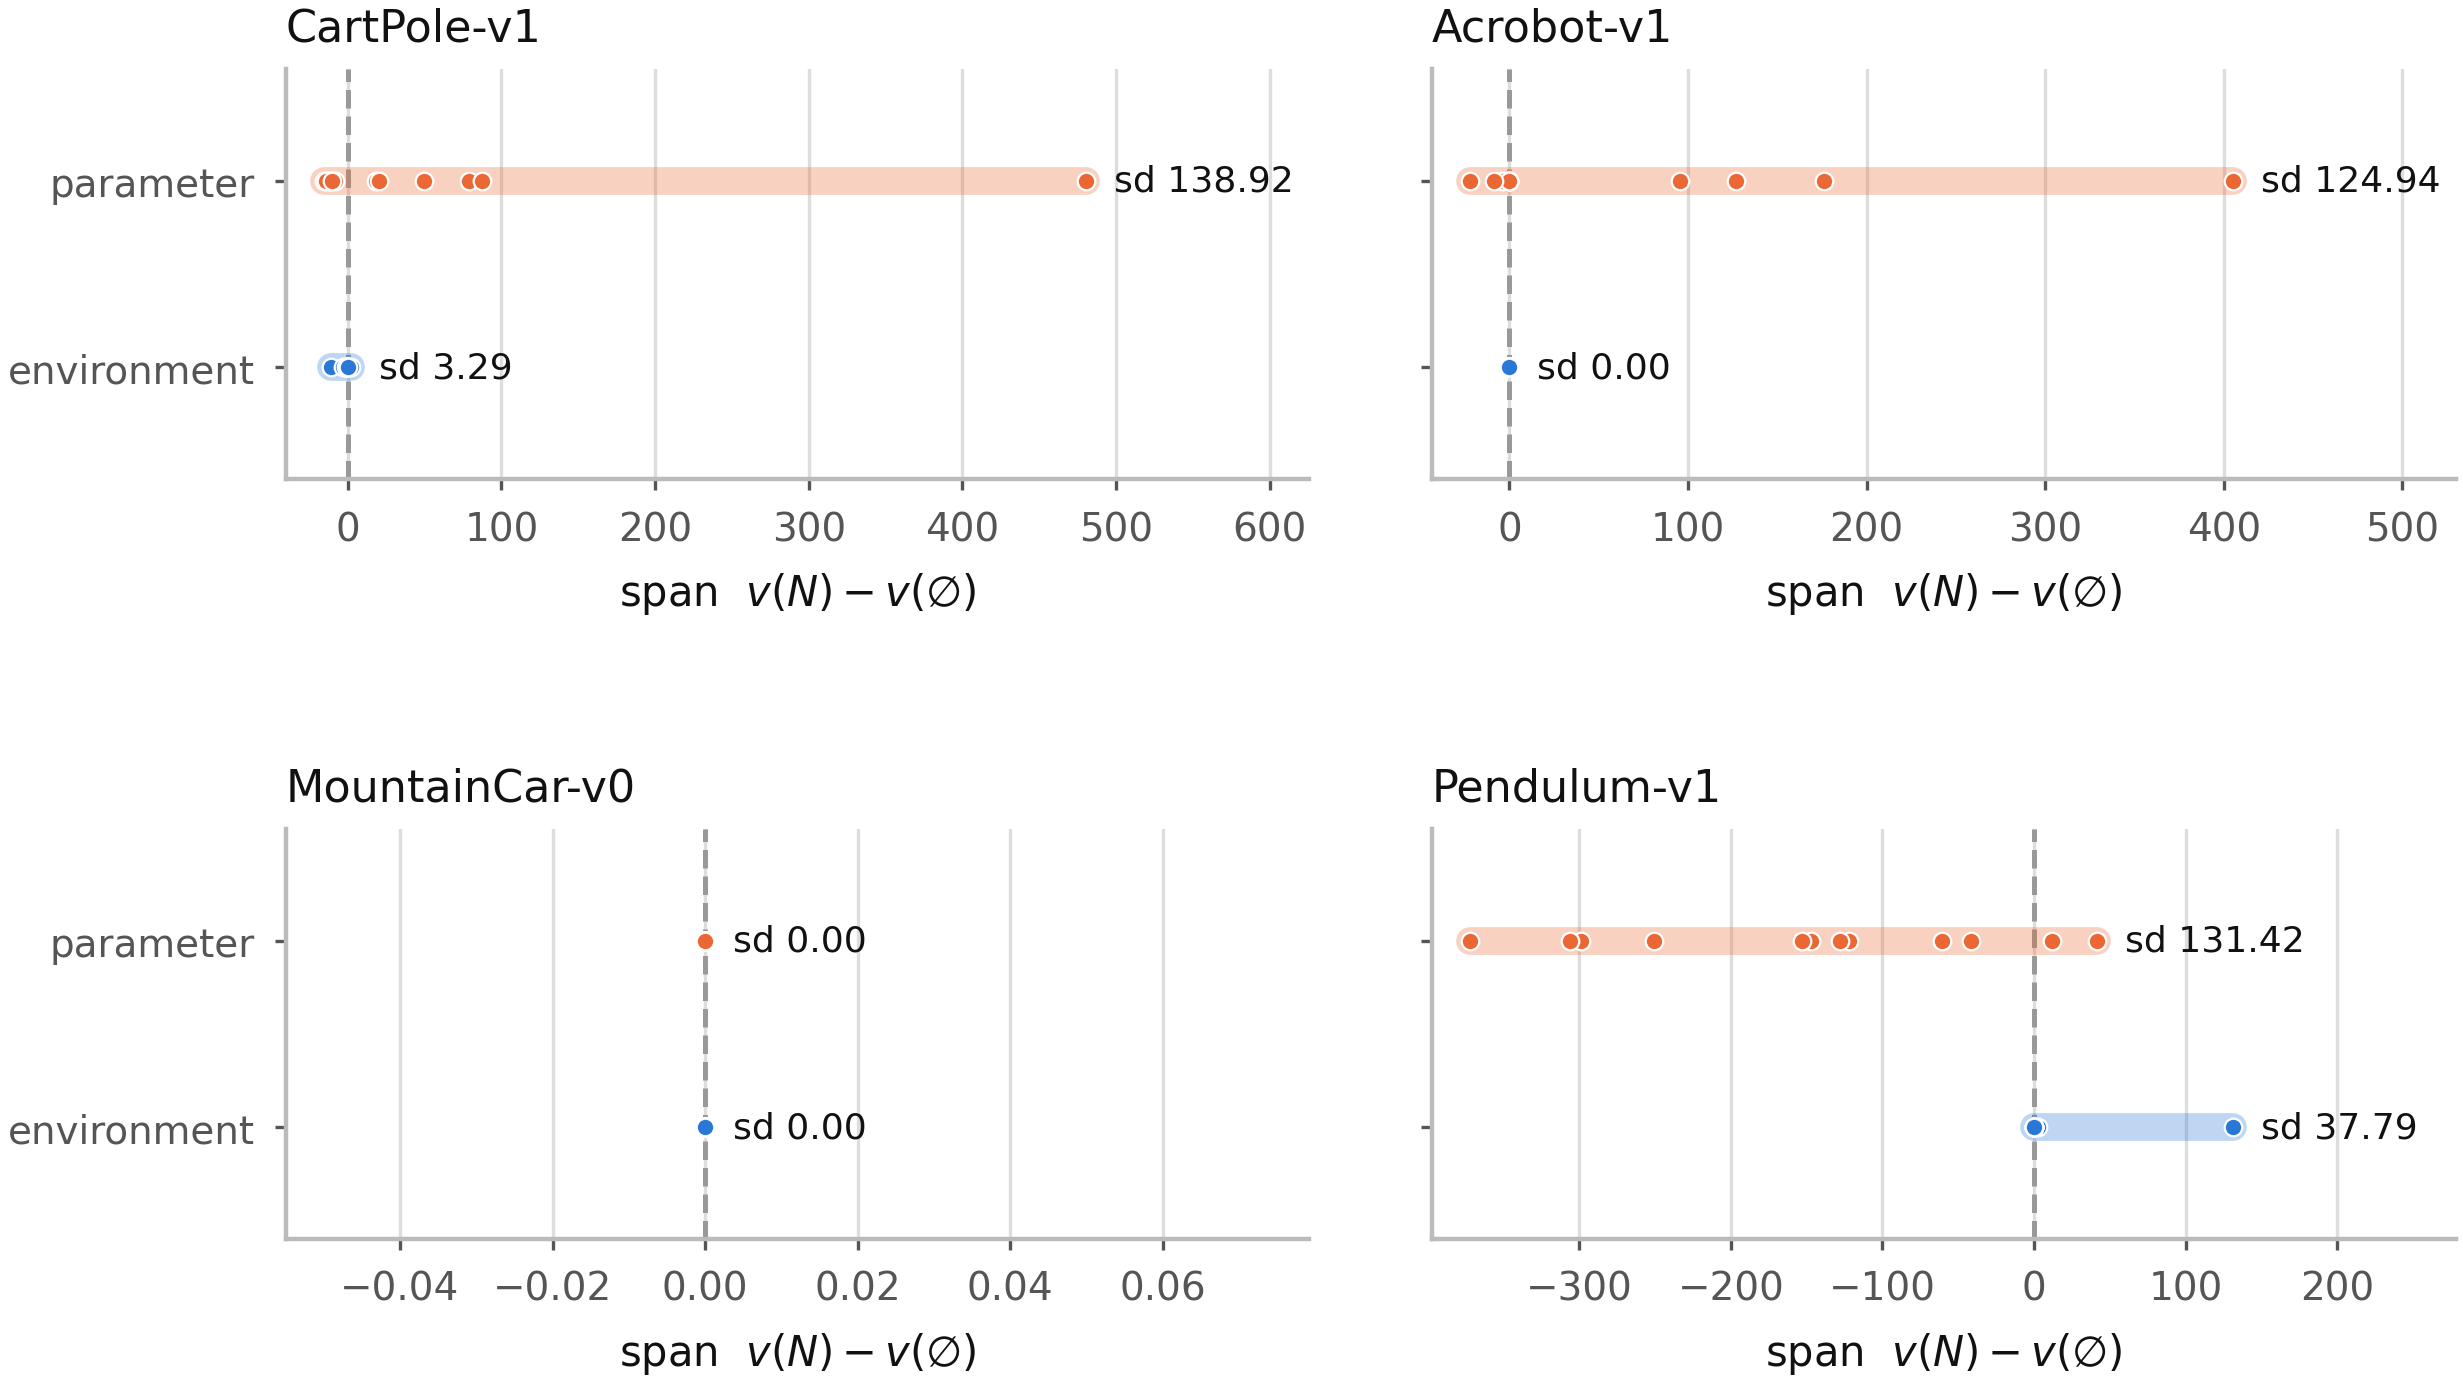
\includegraphics[width=\textwidth]{figures/fig_null_comparison.png}
\caption{Spread of each null construction on four control tasks. Width
determines power: a very wide reference distribution cannot reject anything.
MountainCar is degenerate under both constructions, because no policy in the
budget ever reaches the goal.}
\label{fig:nullcmp}
\end{figure*}

A randomly initialised policy behaves arbitrarily, so masking its inputs moves
return unpredictably and the reference distribution is very wide. The resulting
test has almost no power. Across sixteen checkpoints the parameter null never
exceeds $z=2.45$, including on a converged CartPole policy scoring 404 of 500,
while the environment null reaches $z=+117.6$. The two disagree on five of the
sixteen. The choice of null is not a detail; it decides the verdict, and the
incumbent construction is the one that fails.

Two environments qualify the claim rather than extend it. MountainCar is
degenerate under \emph{both} constructions, at $0.00 \pm 0.00$: within our step
budget no policy ever reaches the goal, every episode returns $-200$, and there
is genuinely nothing to explain. The test declines, correctly, and contributes
no evidence either way. Pendulum narrows the gap to $3\times$ because its
environment null is itself wide ($37.79$): a blind agent on a dense-reward
continuous task still varies in return. The $42\times$ figure is the extreme
case, not the typical one.

Acrobot additionally shows the test tracking \emph{whether there is anything to
explain} rather than agent quality. Its agent fails completely until it learns
($-500$ at $10\%$, $25\%$, $50\%$ of training), the span is exactly $0.00$ there,
and the test correctly declines. CartPole behaves differently because its
observations matter at every skill level. We do not claim undertrained agents
generally produce empty explanations; they do not.

\paragraph{Why the parameter null is wide.}
\label{par:why}
The gap has a mechanism, and it is not about explanations at all. Recording each
random network's \emph{unmasked} return alongside its span
(Figure~\ref{fig:conjecture}) shows the parameter null's width is, to three
significant figures, the spread of random-initialisation return: $138.38$ against
$138.92$ on CartPole, $123.04$ against $124.94$ on Acrobot, $135.49$ against
$131.42$ on Pendulum, and $0.00$ against $0.00$ on MountainCar.

The reason is visible in the decomposition $\Delta = \vfn(N) - \vfn(\emptyset)$.
For a randomly initialised network the masked term is nearly constant across
draws (its standard deviation is $1.8\%$ of the unmasked term's on CartPole and
$5.4\%$ on Acrobot) because a policy that was not using its observations
loses almost nothing when they are removed. The span therefore inherits the
variance of the unmasked term entire. \emph{Parameter randomisation measures the
variance of initialisation, not anything about the explanation being tested},
which is why its reference distribution is wide wherever random networks vary
and why a test built on it has no power. An environment null does not have this
problem because its agents are trained to convergence and land near a common
blind-optimal return.

\begin{figure}[t]
\centering
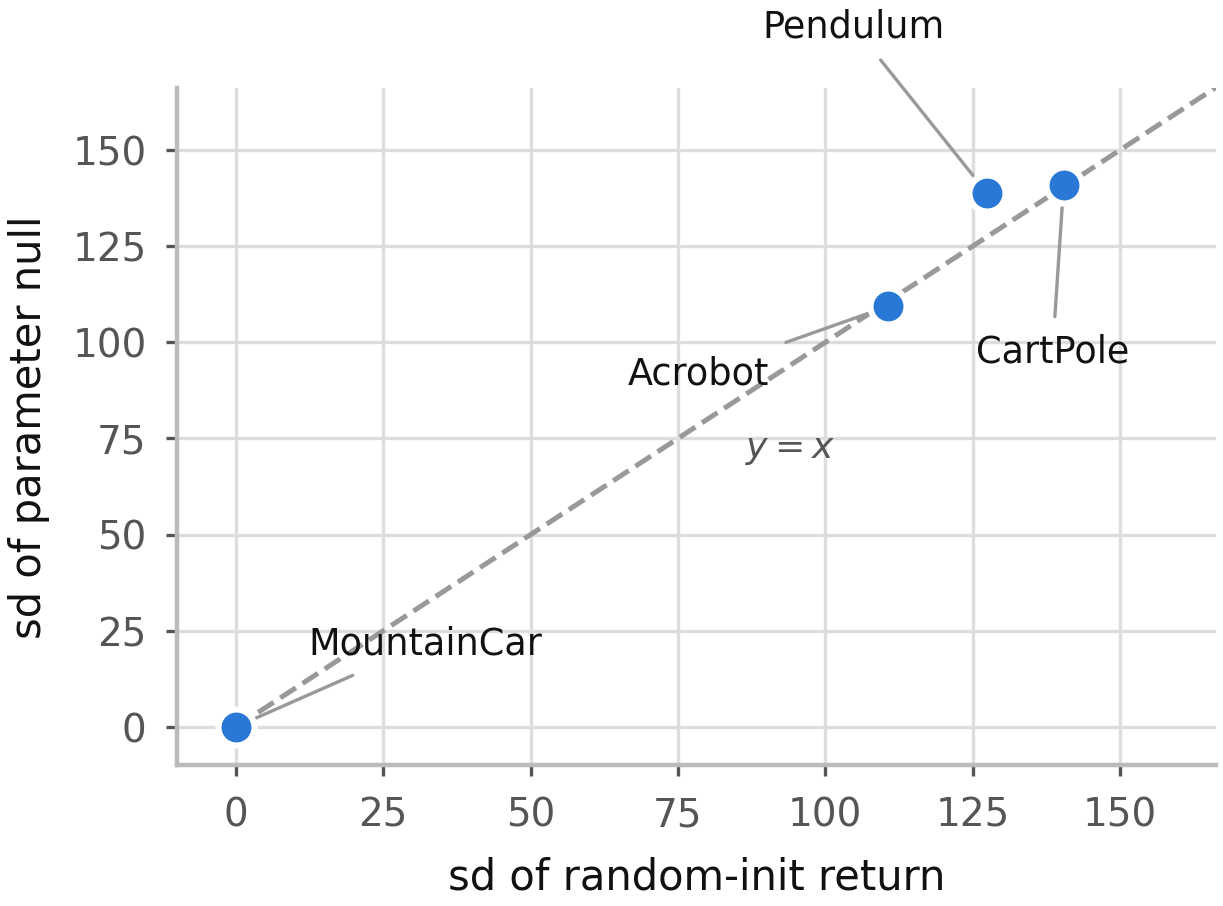
\includegraphics[width=\columnwidth]{figures/fig_conjecture.png}
\caption{The parameter null's width against the spread of random-initialisation
return, one point per environment. The points lie on $y=x$: the established
null's reference distribution is the variance of initialisation.}
\label{fig:conjecture}
\end{figure}

This supersedes the conjecture we offered in an earlier draft, that the width
depended on how often a random network is accidentally competent. That is
roughly right but imprecise: what matters is not competence but \emph{variance}
in competence, and the relationship is an identity rather than a tendency. Four
environments is too few to fit anything, and we report the correspondence rather
than a correlation coefficient for that reason.

\subsection{Attribution is not identified by behaviour}
\label{sec:steering}

We add an auxiliary penalty during training on the divergence between
$\pi(\cdot\mid s)$ and $\pi(\cdot\mid s')$, where $s'$ has one feature resampled
from the batch marginal: the same interventional perturbation the attribution
measures (Table~\ref{tab:steer}, Figure~\ref{fig:steer}).

\begin{table}[t]
\centering\small
\caption{Steering one feature's attribution.}
\label{tab:steer}
\begin{tabular}{lrrr}
\toprule
Corpus & Attribution & Return & $p$ \\
\midrule
market          & $39.9\% \to \mathbf{3.2\%}$ & $-3.49 \to -1.65$ & $\mathbf{0.66}$ \\
planted signal  & $46.5\% \to \mathbf{1.5\%}$ & $+45.04 \to \mathbf{+7.92}$ & $<$0.001 \\
\bottomrule
\end{tabular}
\end{table}

\begin{figure*}[t]
\centering
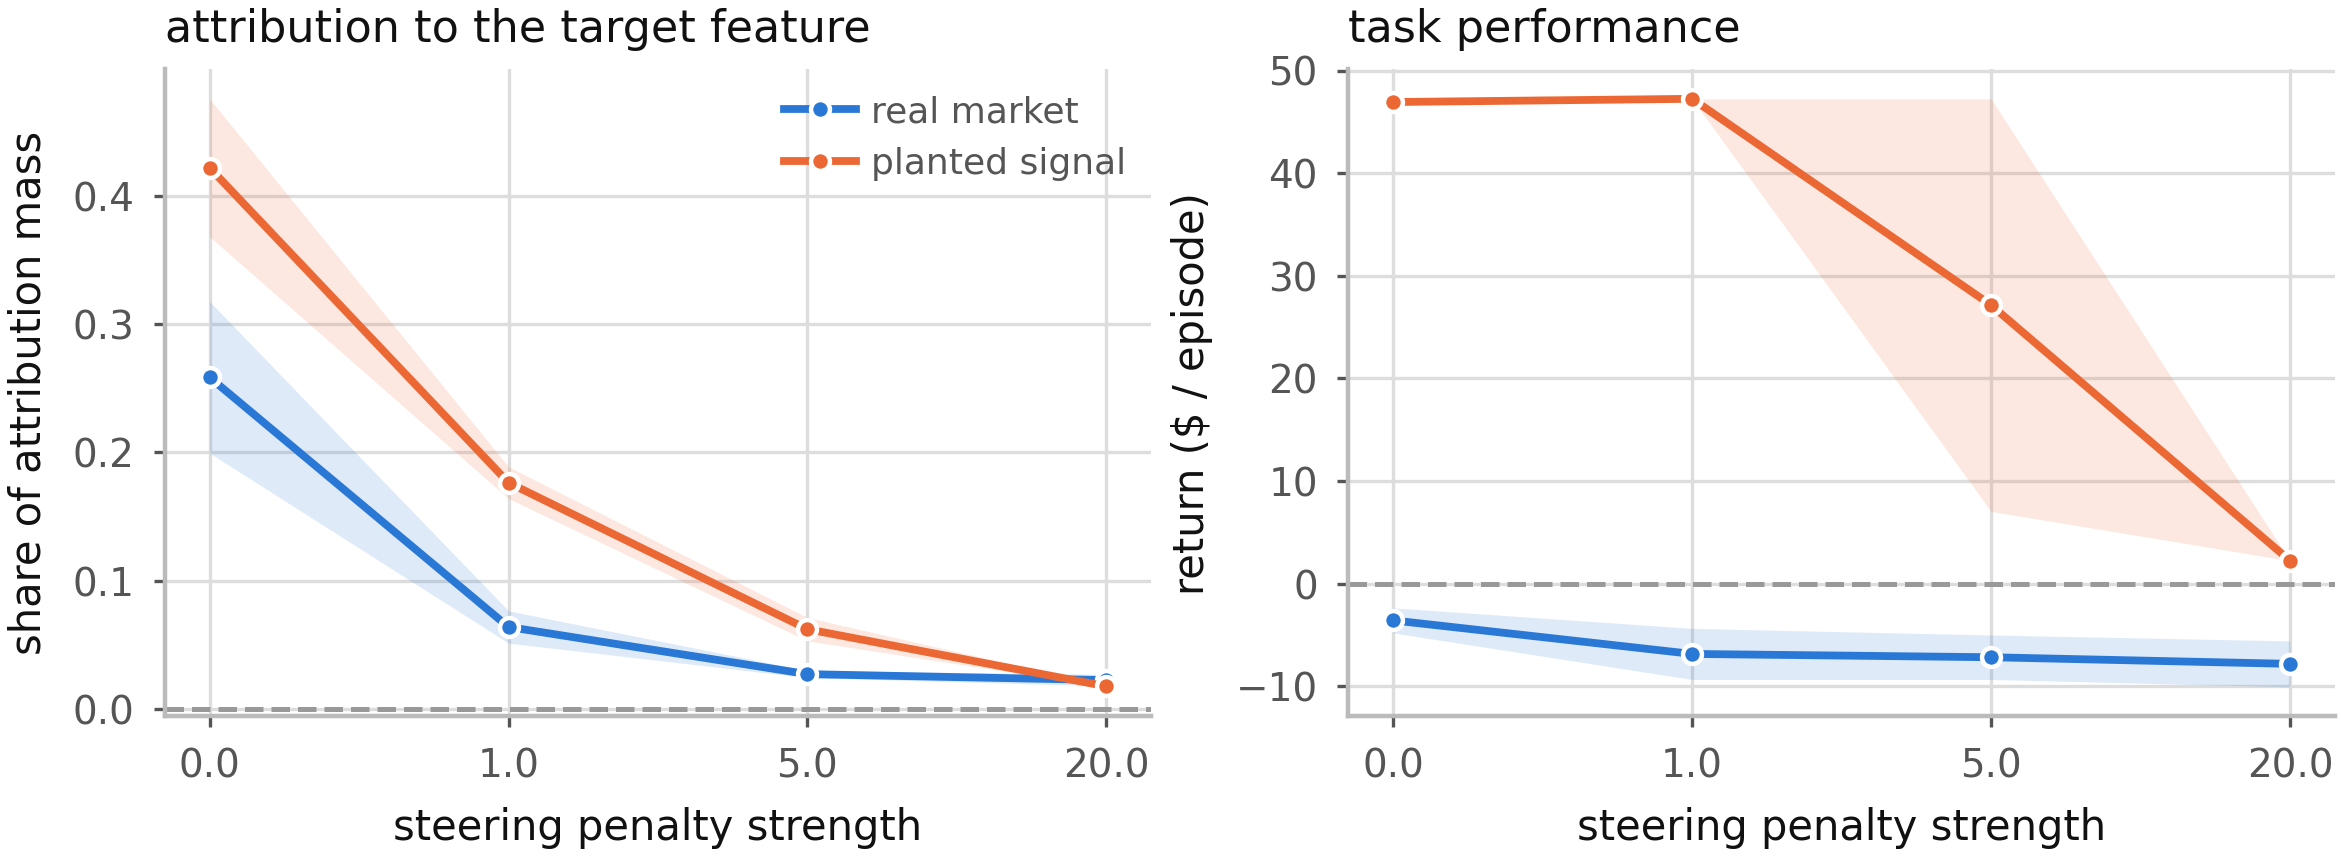
\includegraphics[width=\textwidth]{figures/fig_steering.png}
\caption{Attribution is equally suppressible on both corpora (left). Only where
the feature is load-bearing does suppressing it cost return (right).}
\label{fig:steer}
\end{figure*}

The attribution is equally suppressible in both cases ($92\%$ and $97\%$). What
differs is the price: where the feature is the planted signal, suppressing it
destroys $81\%$ of return; on the market it costs nothing measurable.
Explanations are steerable at no cost exactly where they are not tracking
anything, corroborating Section~\ref{sec:empty} by a route sharing no machinery
with the null test. The control matters: had steering succeeded on both corpora,
the penalty would merely be defeating the attribution method.

\subsection{What the verdict does and does not depend on}
\label{sec:robust}

\paragraph{Attribution family.} Integrated gradients~\citep{sundararajan2017axiomatic},
sharing no machinery with Shapley, ranks features at $0.981$ correlation with Shapley across five seeds and
is comparably seed-stable ($0.750$ against $0.800$). Per-feature attributions are
not a Shapley artefact. IG cannot test the outcome-level claim: episode return is
not differentiable through the environment, so IG has no outcome analogue. Its
behaviour-level span reports the market agent as informative ($z=+4.58$), which
is consistent rather than contradictory and is precisely the
behaviour-versus-outcome distinction of \citet{beechey2023sverl}. The agent's
behaviour does respond to its observations; that responsiveness earns nothing.

\paragraph{Credit assignment.} Leave-one-out ($\vfn(N)-\vfn(N\setminus i)$) and
only-one-in ($\vfn(\{i\})-\vfn(\emptyset)$) are the extremes of the average
Shapley takes, and neither satisfies efficiency, so each carries its own total.
On the planted signal all three fire ($z = +10.66$, $+10.96$, $+2.29$); on the
market none does ($z = -0.42$, $-1.57$, $-0.72$). The verdict is
scheme-independent. \emph{The per-feature ranking is not}: leave-one-out and
only-one-in rank features at only $0.309$ correlation with each other on the same
agent. Whether there is anything to explain is robust; which features matter is
not, and a ranking from a single scheme should not be reported as the answer.

\paragraph{Horizon.} We hypothesised that the parameter null's excess variance
arises because randomising weights perturbs the measurement's \emph{domain},
return being a functional of the policy-induced state distribution, and that this
compounds along the trajectory. The prediction is that its variance grows with
horizon faster than the environment null's. It does not: over horizons 4 to 28
both grow near-linearly at indistinguishable rates ($\alpha=0.94$, $r^2=0.995$
against $\alpha=0.83$, $r^2=0.998$), the ratio flat at $1.7$--$1.8\times$. The
hypothesis is rejected. The gap is instead accounted for by the
initialisation-variance identity of Section~\ref{sec:nulls}, which involves no
compounding along the trajectory and is consistent with the flat ratio found
here.

The experiment did establish something else. At horizon 56 the environment null
collapses to a standard deviation of $0.04$ with two distinct values across
sixteen agents: every blind agent converged on the same abstaining policy. This
is the Acrobot degeneracy again, and it now has a mechanism: the environment null
degenerates when the task affords enough time to learn that inaction is optimal.

\subsection{Off-manifold masking}
\label{sec:manifold}

The standard objection to perturbation attribution applies here and deserves a
direct answer. We define $\vfn(S)$ by replacing the features outside $S$ with
draws that ignore the features inside $S$. Our 18 market features are
correlated, so those draws break the joint distribution and the policy is scored
on states that never occur. \citet{slack2020fooling} build their attack on
precisely that gap. If the span reflected distribution shift rather than
information, the headline result would be an artefact of the masking.

\begin{figure}[t]
\centering
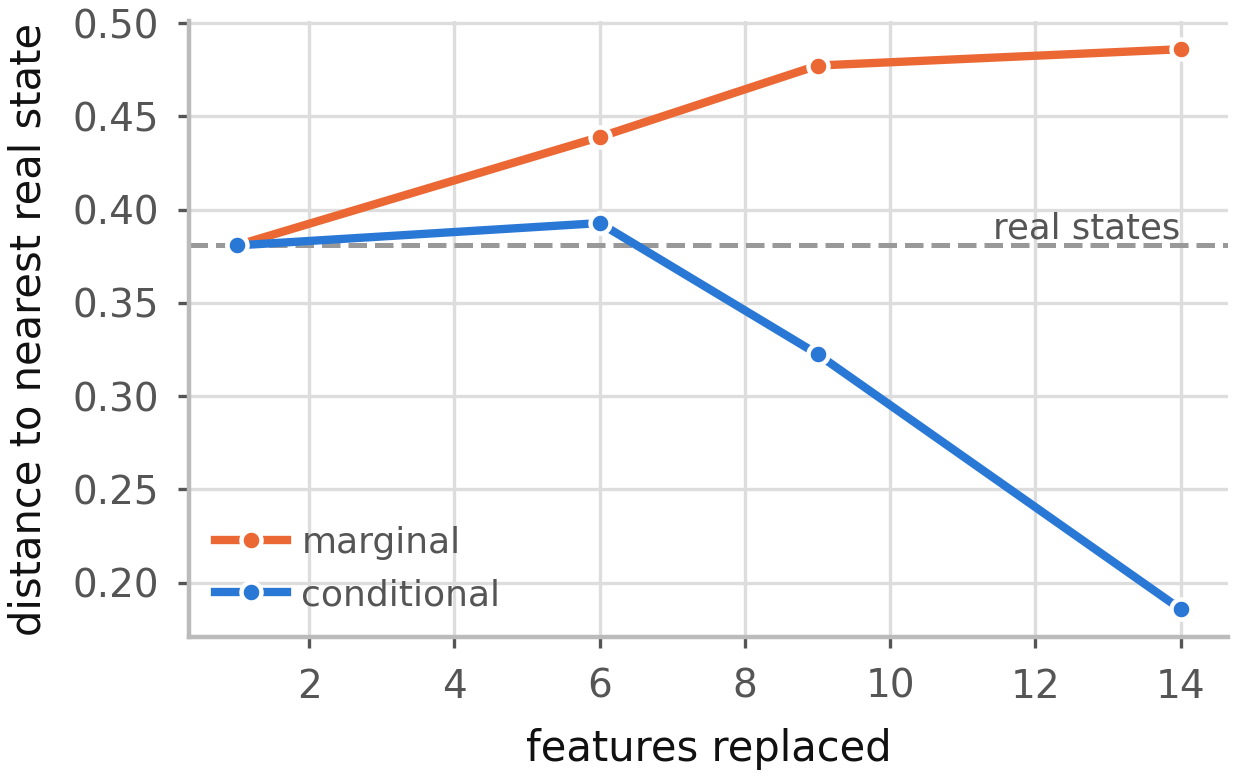
\includegraphics[width=\columnwidth]{figures/fig_manifold.png}
\caption{Distance from a masked state to the nearest real state, in per-feature
standard deviations, against the number of features replaced. The dashed line is
where real held-out states sit relative to the reference sample. Marginal
masking moves \emph{above} that floor as more features are replaced;
neighbour-conditioned masking stays at or below it. The fully-masked point is
omitted: those states are drawn from the reference sample itself, so their
distance to it is zero by construction rather than by evidence.}
\label{fig:manifold}
\end{figure}

\paragraph{The span cannot be an off-manifold artefact.}
This is structural rather than empirical, and we state it as such. The statistic
is $\Delta = \vfn(N) - \vfn(\emptyset)$, and neither coalition evaluates an
off-manifold state. $\vfn(N)$ masks nothing. At $\vfn(\emptyset)$ our
implementation replaces the entire observation from a \emph{single} reference
row, so the synthetic state is itself a real observation, merely a different
one. Conditioning is vacuous on an empty kept set, since
$p(x \mid \emptyset) = p(x)$. A conditional masker must therefore agree with the
marginal one on $\Delta$ exactly, and ours does: $+8.838$ under both. That
equality confirms the implementation respects the argument; it is not
independent evidence for it.

\paragraph{The concern is real in the interior.}
It would be convenient but false to stop there, because the argument above says
nothing about intermediate coalitions, which is where per-feature attributions
live. We implemented a conditional masker that draws replacements from the $k=16$
reference rows nearest the current state in the kept features only, approximating
$p(x_{\bar S} \mid x_S)$. Measuring the distance from masked states to the
nearest real state (Figure~\ref{fig:manifold}) shows the two modes are not
equivalent: with 14 of 18 features replaced, marginal masking sits at $0.486$
against a real-state floor of $0.381$, while conditional masking sits at $0.186$.
Marginal masking does leave the manifold, by a measurable amount, in the interior.

\paragraph{Consequences.}
Re-deriving the verdict entirely under conditional masking, against a null of 12
conditionally-masked blind agents, reproduces it: the planted signal fires at
$z=+9.61$ and the real market does not at $z=-0.55$. The per-feature ranking is
another matter. Leave-one-out values under the two modes correlate at only
$0.767$ by rank, and \emph{they disagree on which feature is most important}.
This is the same split Section~\ref{sec:robust} found for credit assignment:
whether there is anything to explain is robust, which feature to name is not. A
practitioner may report the verdict; the ranking should carry the masking mode
with it.

\subsection{Reproduction from scratch}
\label{sec:repro}

All figures above come from a corpus rebuilt after deleting every cached file. An
earlier corpus, collected five days before and sharing $93\%$ of its contracts,
gave PPO $-0.418 \pm 0.260$ ($p=0.129$) against $-0.595 \pm 0.176$ ($p=0.100$),
and null-test $z$ of $+12.27 / +0.72 / -0.15$ against $+12.27 / +0.72 / +0.23$.
Every conclusion is identical on both. Buy-and-hold moved from $+0.068$ to
$-1.608$, confirming its earlier positive figure reflected that period's $52.3\%$
outcome rate rather than an edge.

\subsection{A positive control on real data}
\label{sec:positive}

Every case where the test fires elsewhere in this paper is synthetic, which
invites the obvious objection: perhaps it detects planted signal rather than
information, and would decline on any real corpus. The control holds the
corpus, the 18 features, the normalizer, the walk-forward split and the null
construction fixed, and varies only the objective.

The market's implied probability is well calibrated, with a weighted mean
absolute error of $0.0172$. A calibrated price is highly informative
\emph{about the outcome} while offering nothing to trade against, because the
fee schedule takes more than the edge. So we score the same agent architecture
on the same real episodes for \emph{calling} the settlement rather than trading
it: $+1$ for each step the call agrees with the eventual outcome, $-1$ when it
disagrees, $0$ for abstaining. Reward may reference the settlement; an
observation may not, and none does. The environment subclasses the trading one,
so the observation construction and normalizer handling are literally the same
code and a difference in results cannot be a difference in the environment.

Against a null of 24 agents trained on these same real episodes with the
observation channel blinded, the prediction agent's span is $+7.46$ against a
null of $-0.48 \pm 2.34$, giving $z=+3.40$: informative, and unchanged in every
one of 4{,}000 resamples. The trading agent on the identical episodes, against
the identical null construction, gives $+7.41$ against $+2.47 \pm 2.29$ and
$z=+2.16$, which the two-part rule declines. Note that the two spans are almost
the same size; what separates them is the null. A blind agent cannot call the
outcome at all, so the prediction null sits at zero, while a blind agent can
still avoid trading and so retains most of the trading agent's advantage.

The same feature stream therefore carries usable information for one objective
and not for the other, and the test says so. This also sharpens what the
negative result means. It is not that the market data is uninformative; a
calibrated price is very informative. It is that the information is not
\emph{monetisable} through a fee schedule that charges $9\%$ round trip, and an
attribution of the trading agent cannot tell those two situations apart.

\subsection{Our own null construction, checked}
\label{sec:nullchoice}

Section~\ref{sec:nulls} argues that the choice of null decides the verdict and
that practitioners do not check it. That argument applies to this paper, so we
checked.

Section~\ref{sec:method} defines the null as corrupting the observation channel
while leaving dynamics and reward intact. The null used for the market result
does something slightly different: its agents are trained \emph{and} attributed
on synthetic signal-free corpora, so the corpus changes as well as the
information, and their spans are measured on synthetic episodes while the
observed span is measured on real ones. The two quantities being compared are
not measured on the same thing.

\begin{figure}[t]
\centering
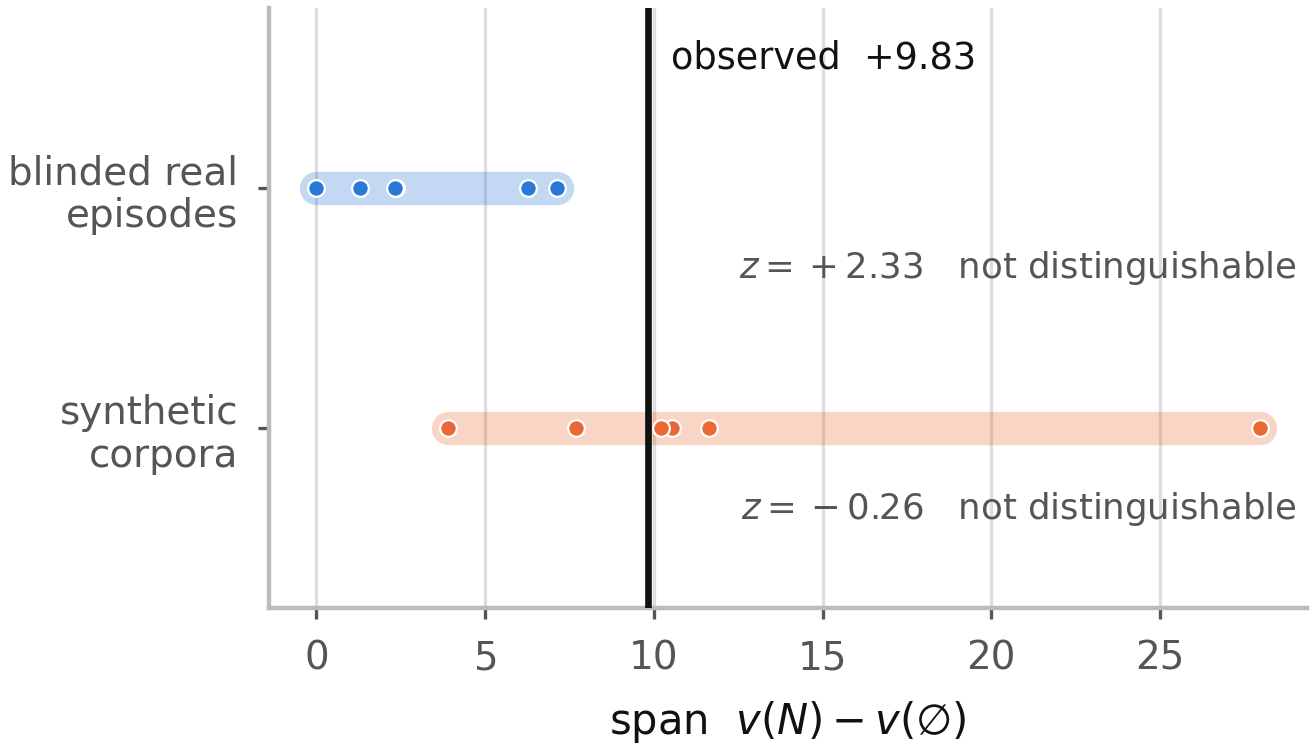
\includegraphics[width=\columnwidth]{figures/fig_nullchoice.png}
\caption{One agent, one observed span, two null constructions. The vertical
line does not move; only the reference distribution does. The synthetic-corpus
null is nearly twice as wide, because it absorbs corpus-to-corpus variation the
observation does not have.}
\label{fig:nullchoice}
\end{figure}

We therefore rebuilt the null the way the method section defines it: agents
trained on the \emph{real} training episodes with observations replaced by
moment-matched noise, and attributed on the same real test episodes as the
observation. Holding the agent fixed at the checkpoint the paper explains and
the measurement corpus fixed at the real test split, the null construction is
then the only thing that varies (Figure~\ref{fig:nullchoice}, $n=32$ each).
Section~\ref{sec:matched} applies the same correction to every case rather
than to this one alone, and reports what it costs:

\begin{center}\footnotesize
\begin{tabular}{lrrl}
\toprule
Null & Mean $\pm$ sd & $z$ & Verdict \\
\midrule
synthetic corpora & $+9.07 \pm 4.91$ & $-0.34$ & not distinguishable \\
blinded real & $+2.26 \pm 2.21$ & $+2.33$ & not distinguishable \\
\bottomrule
\end{tabular}
\end{center}

The verdict survives, but not comfortably, and the reason it survives is worth
stating. Under the blinded-real null the normal statistic \emph{does} reject at
$z=+2.33$; the rank statistic does not, and Section~\ref{sec:method} requires
both. The two-part rule is doing real work here rather than being a formality.

Resampling each null (Section~\ref{sec:intervals}) shows how much weight the two
comparisons carry. The synthetic-corpus verdict is unchanged in $100\%$ of
replicates; the blinded-real verdict in $65\%$.

At this point we intended to adopt the blinded-real construction throughout, on
the argument just given. Section~\ref{sec:matched} reports why we did not: run
on every case rather than on this one, it produces a false positive on a corpus
built to contain no signal. The argument above is right about what the null
should hold fixed and wrong about how to hold it, and we would not have found
that by reasoning further about it.

An earlier run of this comparison at $n=12$ put the two constructions on
opposite sides of the threshold. That disagreement was a small-sample artefact
and disappeared at $n=32$. We mention it because it is the failure mode this
paper is about, encountered in our own results, and because $n=12$ null agents
is a common budget.

\subsection{Confidence intervals on the verdicts}
\label{sec:intervals}

Every $z$ in this paper divides by a standard deviation estimated from 12 to 32
null agents. Reporting it to two decimals hides that. We resample the null
draws with replacement and re-apply the full two-part decision rule to each
replicate, which gives a percentile interval for $z$ and, more usefully, the
fraction of replicates in which the verdict is unchanged.

Every verdict in the paper is stable in $100\%$ of replicates except the two
blinded-real market comparisons, at $64\%$ and $65\%$.
The planted signal's interval is $[+10.3, +16.9]$ and the market's, under the
null used in Section~\ref{sec:empty}, is $[-0.16, +0.73]$: nowhere near the
threshold in either direction. This bootstraps the null only. Uncertainty in the
observed statistic, a mean over held-out episodes, is not included, so these
intervals are optimistic in a way we would rather state than hide.

\subsection{Correcting the null everywhere, and why we did not}
\label{sec:matched}

Section~\ref{sec:nullchoice} argues that a null should hold the corpus fixed and
vary only the information. Taken seriously that is a per-case construction: for
each case, train the null agents on \emph{that} case's episodes with the
observation channel blinded, and attribute them on the same rollout as the
observation. We built it and ran all three cases. It cannot be used.

\begin{center}\footnotesize
\begin{tabular}{lrrrl}
\toprule
Case & Span & Null & $z$ & Verdict \\
\midrule
planted signal & $+74.69$ & $0.00 \pm 0.00$ & $+\infty$ & fires \\
\textbf{null corpus} & $\mathbf{+13.90}$ & $0.00 \pm 0.00$ & $+\infty$ &
\textbf{fires} \\
real market & $+7.40$ & $2.97 \pm 2.29$ & $+1.93$ & declines \\
\bottomrule
\end{tabular}
\end{center}

The middle row is a corpus constructed to contain no informative feature. The
test fires on it. The construction has power and no specificity, and a test with
no specificity is not a test.

\paragraph{The two nulls are not the same null.}
The mechanism explains the original design better than the original design
explained itself. A \emph{signal-free corpus} gives agents that can see, in an
environment whose observations carry no information about the outcome; they
still respond to observational structure, so their spans are nonzero and spread
out. A \emph{blinded channel} gives agents that cannot see; they converge to a
constant policy, and a constant policy's return does not depend on its inputs at
all, so every null span is exactly zero.

The agent under test is sighted. The correct reference is therefore sighted
agents with nothing to learn, not blind ones. Blinding removes the agent's
capacity to respond to observational structure along with the information, and
the null collapses onto a point mass at zero against which any nonzero span is
declared significant. This is why the degeneracy noted in
Section~\ref{sec:method} is a defect rather than a strong result, and why the
Acrobot degeneracy in Section~\ref{sec:nulls} should be read as a warning about
the reference rather than as a curiosity.

\paragraph{The collapse is a matter of convergence.}
On the synthetic corpora the null is a point mass; on the real market it has
width $2.29$. That difference is not about the corpora but about how far the
blind agents got. The real training split is roughly four times the size of the
synthetic ones, so the same 40 updates is a quarter as many passes over the
data. Sweeping the null agents' budget with everything else fixed
(Figure~\ref{fig:budget}) shows the null closing on zero as their return
approaches abstention, and the verdict on the real market changing with it:

\begin{center}\footnotesize
\begin{tabular}{rrrrl}
\toprule
Updates & Null mean $\pm$ sd & $z$ & Blind return & Verdict \\
\midrule
20 & $+5.60 \pm 3.27$ & $+0.55$ & $-8.74$ & declines \\
40 & $+3.55 \pm 2.25$ & $+1.71$ & $-4.13$ & declines \\
80 & $+0.55 \pm 1.62$ & $\mathbf{+4.23}$ & $-0.18$ & \textbf{fires} \\
160 & $-0.02 \pm 0.04$ & $\mathbf{+203.6}$ & $-0.05$ & \textbf{fires} \\
\bottomrule
\end{tabular}
\end{center}

So the construction does not merely fail on synthetic corpora. Trained to
convergence it reports the market agent's explanation as informative at
$z=+203.6$, which is the opposite of what every other measurement in this paper
says, and it does so for a reason that has nothing to do with the agent: the
null's standard deviation has fallen from $3.27$ to $0.04$ while the observed
span has not moved at all. A reference distribution that tightens with its own
training budget cannot be read as a property of the agent under test, and a test
whose verdict is set by that budget is measuring the budget.

\begin{figure}[t]
\centering
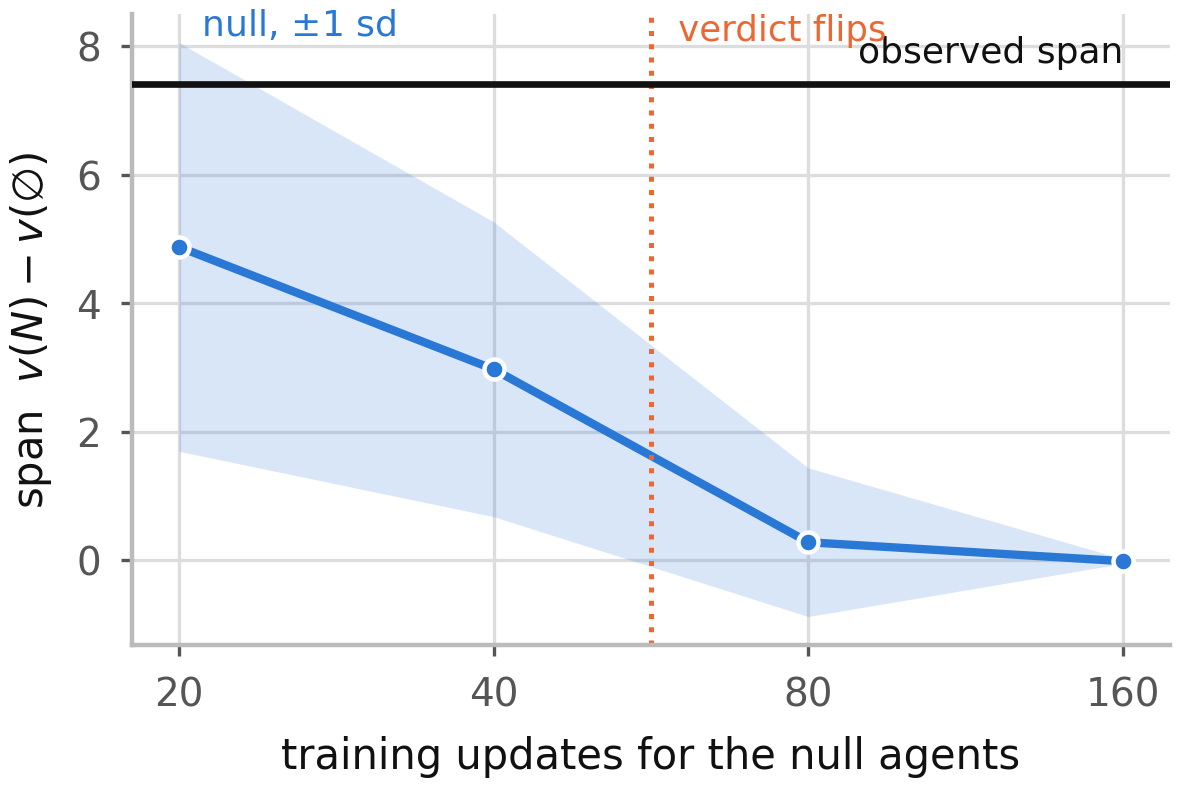
\includegraphics[width=\columnwidth]{figures/fig_budget.png}
\caption{The blinded null collapses as its agents converge on abstention. The
observed span is fixed; only the reference moves. A null that tightens with its
own training budget cannot be read as a property of the agent under test.}
\label{fig:budget}
\end{figure}

\subsection{A third construction, and a pattern}
\label{sec:permuted}

Section~\ref{sec:matched} leaves an obvious gap: hold the corpus fixed
\emph{and} keep the null agents sighted. There is a natural way to do it, and it
is the construction this paper claimed to be supplying all along. Permute the
outcomes across episodes and leave everything else alone. The observation stream
is untouched, because the feature block is a function of the quote and spot
arrays and never reads the settlement, so no observation moves by a single bit.
The marginal outcome rate is preserved exactly, since a relabelling is not a
resample. This is the direct analogue of the label-permutation test of
\citet{adebayo2018sanity}.

It has power and specificity (Figure~\ref{fig:constructions}): on the planted
signal it fires at $z=+10.48$, and
on the signal-free corpus it declines at $z=+1.75$. No null collapses. It is
nonetheless unusable, and the way it fails is the most instructive of the three.

\begin{center}\footnotesize
\begin{tabular}{lrrrl}
\toprule
Case & Span & Null & $z$ & Verdict \\
\midrule
planted signal & $+74.69$ & $+11.89 \pm 5.99$ & $+10.48$ & fires \\
null corpus & $+13.90$ & $+7.96 \pm 3.39$ & $+1.75$ & declines \\
\textbf{real market} & $\mathbf{+7.40}$ & $\mathbf{+55.85 \pm 3.12}$ &
$\mathbf{-15.52}$ & \textbf{below null} \\
\bottomrule
\end{tabular}
\end{center}

The market agent's span is not merely inside the reference distribution, it is
fifteen standard deviations \emph{below} it. The null agents earn $+36.26$ per
episode where the observed agent earns $-1.13$. They are not agents with nothing
to learn; they are agents with a great deal to learn.

\paragraph{Permuting a label that the observations forecast.}
The price is a forecast of the outcome. Permuting the outcome leaves the
forecast in place and attaches it to a different contract, so the market becomes
grossly mispriced: a contract whose price has moved to $0.99$ now settles at
$0.49$. Fading the terminal price, a rule needing nothing but the quote, earns
$-0.005$ per contract in the real corpus and $+0.486$ in the permuted one, which
at the position cap is roughly \$49 an episode. Calibration error rises from
$0.007$ to $0.456$.\footnote{Terminal mid on the training split in eight
quantile bins, which is not the estimator behind the figure in
Section~\ref{sec:market}; only the contrast is meant to be read.} The null
agents learn that arbitrage, it requires seeing the price, and their spans
inflate accordingly.

This is not a quirk of prediction markets. \emph{Wherever an observation is a
forecast of the label, permuting the label makes that forecast exploitably
wrong}, and the null agents are handed a task easier than the real one rather
than harder. Supervised learning does not have this problem because the model
does not act on its input and cannot trade against it.

\begin{figure*}[t]
\centering
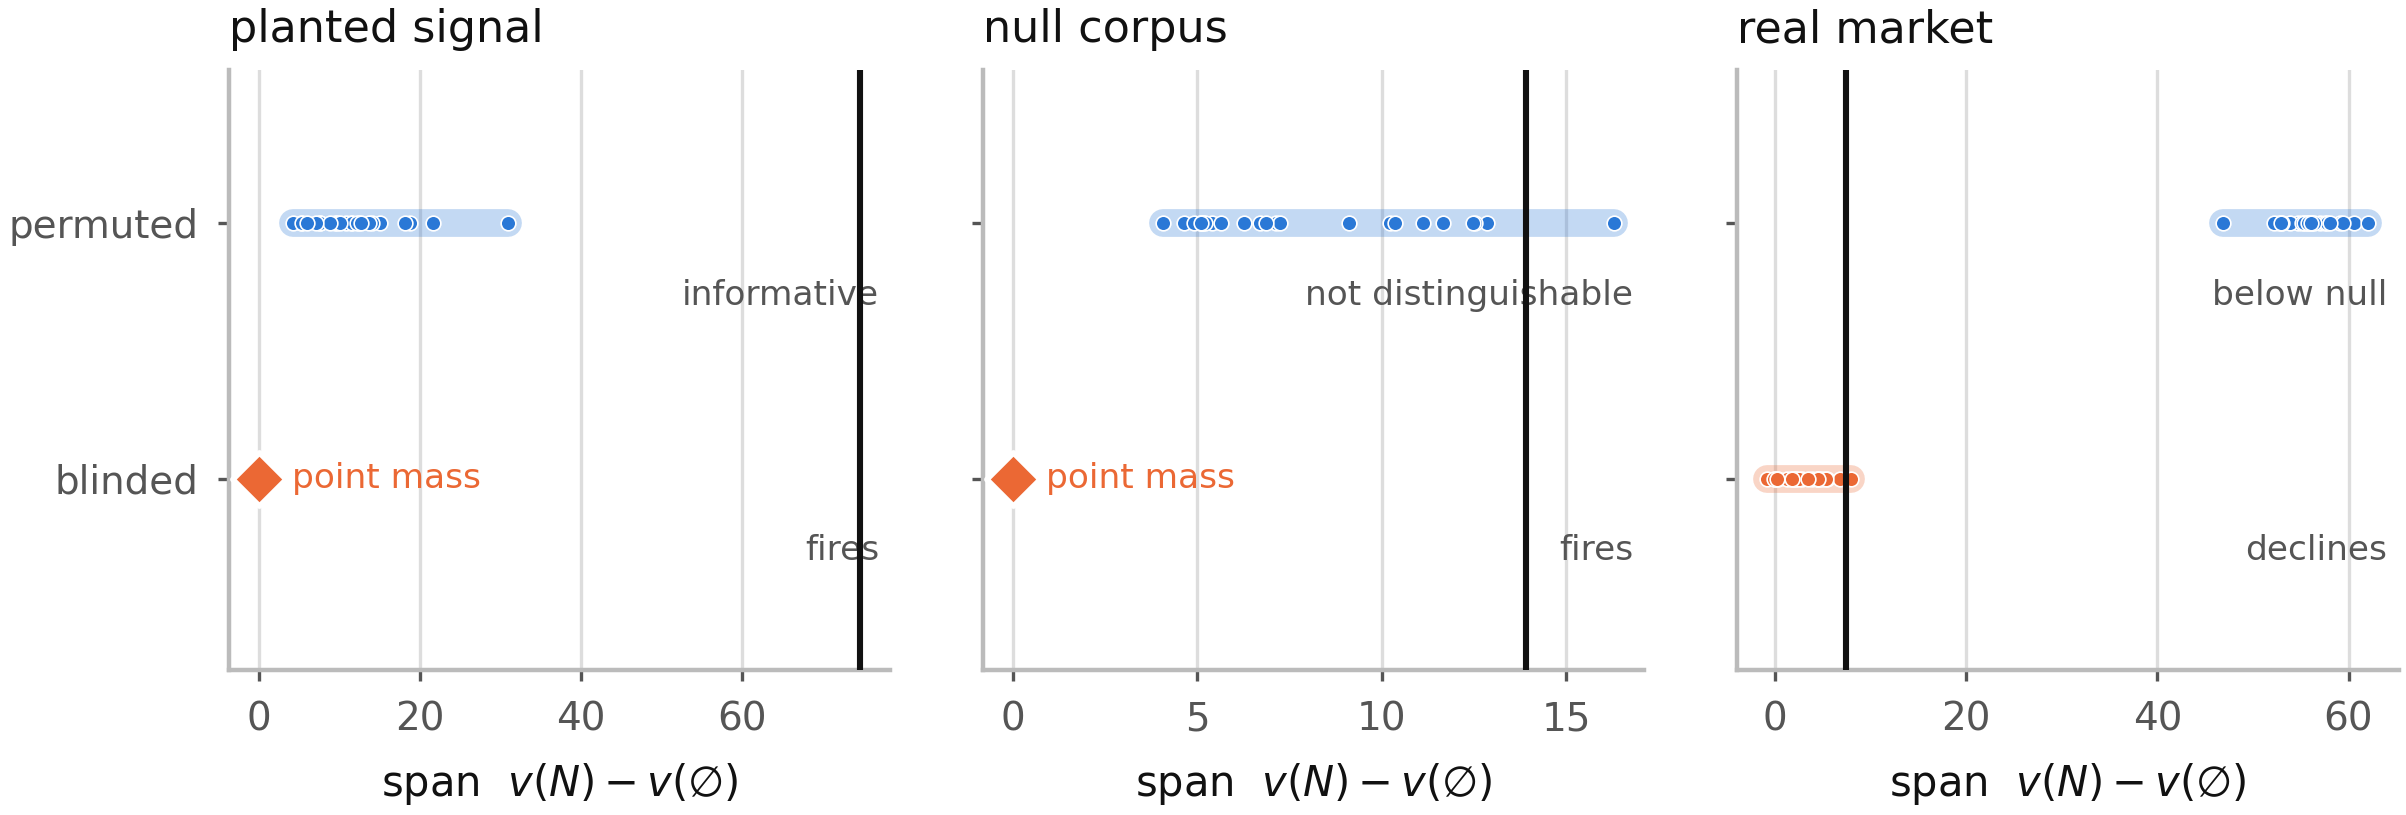
\includegraphics[width=\textwidth]{figures/fig_constructions.png}
\caption{Two null constructions on the same three cases. The vertical line is
the observed span and does not move; only the reference does. Blinding the
observation channel yields a point mass on both synthetic corpora, which is why
it fires on the one built to contain no signal. Permuting the outcomes yields a
usable reference everywhere, and on the real market places it so far above the
observed span that the agent lands fifteen standard deviations below its own
null.}
\label{fig:constructions}
\end{figure*}

\paragraph{The pattern.}
Three constructions, three failures, and the same shape each time. Removing the
information also perturbs something else, and the perturbation decides the
verdict:

\begin{center}\footnotesize
\begin{tabular}{p{0.24\columnwidth}p{0.30\columnwidth}p{0.34\columnwidth}}
\toprule
Construction & Also changes & Consequence \\
\midrule
signal-free corpus & the corpus & widens the reference; errs toward declining \\
\addlinespace
blinded channel & the agent's capacity to respond & collapses to a point mass;
fires on anything, budget-dependent \\
\addlinespace
outcome permutation & the price's calibration & creates an arbitrage; the null
learns more than the agent \\
\bottomrule
\end{tabular}
\end{center}

We report this as the finding rather than presenting a fourth construction we
have not tested. A null for reinforcement learning has to remove the
information while leaving the observation stream, the agent's responsiveness,
and the task's difficulty intact, and none of the three natural ways of doing
that manages all four. \citet{huber2022benchmarking} observed that the
data-randomisation test has no obvious RL analogue. We set out to supply one and
instead have an account of why it is hard.

\paragraph{What we keep.}
The results in this paper use the signal-free-corpus null, whose fault is the
mildest of the three: it widens the reference and so errs toward declining,
which is the conservative direction for every claim we make with it. That is a
reason to trust our negative results more than our positive ones, and we would
not have been able to say which way the bias ran without building the other two.
One construction we have not tried is a \emph{stratified} permutation, shuffling
outcomes only within price buckets, which would preserve calibration and remove
only the information beyond the price. It asks a narrower question, whether the
agent knows anything the market does not, and that may be the better question.

\subsection{Implications for oversight}
\label{sec:oversight}

The case for interpretability as an oversight mechanism is that seeing which
inputs drive a policy tells us something about whether to trust it. Three of
our results bear on that argument, and none of them requires an adversary.

\paragraph{Passing every check is not evidence.}
On a corpus where the correct answer is known to be ``nothing'', an agent's
attribution is stable across seeds, separated beyond its own estimation error,
and semantically legible. Every property a practitioner would check is present
and the explanation is empty. Stability in particular is worth naming: it is
the most commonly reported evidence that an explanation is trustworthy, and
Section~\ref{sec:rejected} records that we expected instability to be the tell
and were wrong. Emptiness and instability are unrelated.

\paragraph{Explanations are cheap to forge, without deception.}
Section~\ref{sec:steering} drives a feature's attribution from $39.9\%$ to
$3.2\%$ of total mass at no measurable cost in return. This needs no deceptive
policy, no attack on the explainer, and no knowledge of who will audit the
model: an auxiliary training term is enough, and the resulting explanation is
\emph{correct} about the resulting agent. The cost of forgery is exactly the
importance of the feature, which is zero for features that do not matter. An
oversight regime that reads attributions as evidence of what a model relies on
is therefore reading a quantity the developer can set, in the region where it
would most want a guarantee.

\paragraph{The verdict depends on a choice nobody reports.}
Section~\ref{sec:nulls} shows the established sanity check has almost no power
in RL. Section~\ref{sec:nullchoice} shows our own headline is sensitive to the
construction, and Section~\ref{sec:matched} shows that the alternative which
looks more principled is broken, in a way visible only by running it rather than
by reasoning about it. A reported attribution is not interpretable without the
reference distribution it was measured against, and that reference is currently
neither standardised nor, in most papers, stated.

\paragraph{What we would ask for.}
Report the null construction alongside any attribution offered as evidence.
Treat a per-feature ranking as a joint property of the attribution scheme and
the masking distribution, since Sections~\ref{sec:robust}
and~\ref{sec:manifold} show it moves under both, to the point of disagreeing on
the most important feature. The aggregate verdict, whether there is anything to
explain at all, is the part that survives; it is also the weaker claim, and it
is the one we would trust.

\subsection{Hypotheses we rejected}
\label{sec:rejected}

Six predictions in this project turned out to be wrong
(Table~\ref{tab:rejected}). They are collected rather than left implicit in the
sections that tested them, because a reader assessing whether the surviving
claims were stress-tested should be able to see what did not survive.

\begin{table*}[t]
\centering\small
\caption{Predictions this project made and then rejected on its own evidence.
None of the surviving results depends on any of them.}
\label{tab:rejected}
\begin{tabular}{p{0.29\textwidth}p{0.29\textwidth}p{0.34\textwidth}}
\toprule
Hypothesis & Prediction & Outcome \\
\midrule
An agent with no edge produces unstable explanations, and instability is the
tell. &
Low cross-seed rank correlation. &
\textbf{Rejected.} $0.850$ mean rank correlation, unanimous on the top feature.
Emptiness and instability are unrelated, which is what makes the empty case hard
to catch. \\
\addlinespace
Outcome-level attribution, being tied to return, is more stable than
behaviour-level attribution. &
Higher cross-seed rank correlation for outcomes. &
\textbf{Rejected, and reversed.} Outcomes reach $0.347$ against behaviour's
$0.850$. Attributing to return is noisier, not steadier. \\
\addlinespace
The parameter null is wide because randomising weights perturbs the
measurement's domain and the error compounds along the trajectory. &
Its variance grows with horizon faster than the environment null's. &
\textbf{Rejected.} Over horizons 4 to 28 both grow at indistinguishable rates
($\alpha = 0.94$ against $0.83$), ratio flat at $1.7$--$1.8\times$. \\
\addlinespace
The parameter null is wide because a randomly initialised network is sometimes
an accidentally competent policy. &
Width tracks how often random policies do well. &
\textbf{Superseded.} Roughly right but imprecise: the width is not related to
competence but \emph{equal} to the standard deviation of
initialisation return (Section~\ref{sec:nulls}). A tendency was replaced by an
identity. \\
\addlinespace
A null that holds the corpus fixed, by blinding the observation channel, is more
principled and should replace the shared signal-free-corpus null. &
The same verdicts against a tighter reference, and more power. &
\textbf{Rejected.} It fires on a corpus built to contain no signal, and its
verdict on the real market flips with the null agents' training budget
(Section~\ref{sec:matched}). Blinding removes the capacity to respond to
observational structure, not only the information. \\
\addlinespace
Permuting the outcomes fixes both faults: the corpus is held fixed and the null
agents stay sighted. &
Power, specificity, and a usable reference on all three cases. &
\textbf{Rejected.} It has power and specificity and still fails. The price
forecasts the outcome, so relabelling makes it exploitably wrong: the null
agents earn $+36.26$ against the observed agent's $-1.13$ and the market's span
lands 15 sd \emph{below} its own null (Section~\ref{sec:permuted}). \\
\bottomrule
\end{tabular}
\end{table*}

One further claim is stated in the paper as structural rather than empirical.
The span's invariance to the masking mode (Section~\ref{sec:manifold}) follows
from the construction, since $p(x \mid \emptyset) = p(x)$; the measured equality
confirms the implementation respects that argument and is not independent
evidence for it. We separate the two because a numerical agreement that must
hold is easily mistaken for one that might not have.

\section{Limitations}

\textbf{The construction is adapted.} The test is the data-randomisation test
of \citet{adebayo2018sanity} with an RL-appropriate null; the outcomes framing is
\citet{beechey2023sverl}'s; deletion-based fidelity is standard.

\textbf{The span measures information in aggregate.} An explanation could clear
the test and still misattribute among features. Section~\ref{sec:robust} shows
the ranking is scheme-dependent even when the verdict is not, and
Section~\ref{sec:manifold} shows it is masking-dependent too, to the point of
disagreeing on the most important feature. Only the verdict survives both.

\textbf{Conditional masking is approximated, not solved.} Our conditional
masker is $k$-nearest-neighbour in the kept features, which is a practical
proxy for $p(x_{\bar S} \mid x_S)$ and inherits the usual difficulties in high
dimension. It is adequate to show the two modes differ; it is not a claim to
have sampled the true conditional. Neither mode fixes the deeper issue that
replacements are redrawn each timestep, so masked \emph{states} are plausible
while masked \emph{trajectories} are not.

\textbf{Temporal credit assignment is named, not solved.} Masking a feature for a
whole episode measures whether it mattered, not when. This is
FastSVERL's~\citep{beechey2025fastsverl} territory.

\textbf{Off-policy attribution is not handled.} Masked coalitions induce a
different policy and therefore a different state distribution; estimates are
on-policy for the masked policy, not counterfactuals about the unmasked one.

\textbf{The width identity is measured on four environments.} The correspondence
between the parameter null's width and initialisation-return variance is close
to exact on each task we ran, and it has a mechanism, but four points cannot
establish a law. We report the correspondence, not a fitted relationship.

\textbf{The null construction is chosen, not derived.} We keep the
signal-free-corpus null because the corpus-matched alternative fails
(Section~\ref{sec:matched}), not because we can show it is optimal. Its known
fault is that it varies the corpus as well as the information, which widens the
reference and biases toward declining. A construction that holds the corpus
fixed \emph{and} keeps the null agents sighted would dominate both, and we do
not have one.

\textbf{Scope.} One real domain and four classic-control tasks; one attribution
family for the outcome-level tests. All four control tasks have small
observation spaces, so nothing here speaks to pixel-based or high-dimensional
agents, where the reference distribution is itself the hard problem. Box2D
environments were deliberately excluded: they require a system-level build
dependency, which would trade the one-command reproduction for one more
observation dimension. Corpus membership is not reproducible across time, though
content is.

\section{Conclusion}

An attribution can be stable, precisely estimated, plausible, and empty. The
checks practitioners apply (consistency across runs, separation beyond
estimation error, semantic legibility) do not detect this, because none of them
ask whether the explained agent learned anything. A null-model test does, using
a statistic the attribution framework already provides, and it separates tasks
rather than datasets: on identical real episodes it fires for an objective the
observations can serve and declines for one they cannot.

Two findings bear on using attributions as evidence. They are cheap to forge,
at a price equal to the importance of the feature being hidden, which is zero
exactly where a guarantee would be worth having, and no deception or attack on
the explainer is required to do it. And the verdict depends on a reference
distribution that is currently neither standardised nor usually reported; the
established construction for reinforcement learning has almost no power, because
its width is the standard deviation of random initialisation rather than
anything about the explanation. We recommend against its use without the
measurement in Section~\ref{sec:nulls}, and we recommend reporting the null
construction alongside any attribution offered as evidence, having found in
Section~\ref{sec:nullchoice} that our own choice was worth checking.

\bibliographystyle{plainnat}
\bibliography{references}

\end{document}
